\documentclass[10pt,twocolumn,letterpaper]{article}

\usepackage{cvpr}
\usepackage{times}
\usepackage{epsfig}
\usepackage{graphicx}
\usepackage{amsmath}
\usepackage{amssymb}
\usepackage{caption}
\usepackage{subcaption}
\usepackage{booktabs}
\usepackage{makecell}
\usepackage{algorithm}
\usepackage{algpseudocode}
\usepackage{siunitx}
\usepackage{float}



% Include other packages here, before hyperref.

% If you comment hyperref and then uncomment it, you should delete
% egpaper.aux before re-running latex.  (Or just hit 'q' on the first latex
% run, let it finish, and you should be clear).
\usepackage[pagebackref=true,breaklinks=true,letterpaper=true,colorlinks,bookmarks=false]{hyperref}

% \cvprfinalcopy % *** Uncomment this line for the final submission

\def\cvprPaperID{0446} % *** Enter the CVPR Paper ID here
\def\httilde{\mbox{\tt\raisebox{-.5ex}{\symbol{126}}}}

\newcommand{\hp}[1]{\textcolor{red}{HP: #1}}

% Pages are numbered in submission mode, and unnumbered in camera-ready
\ifcvprfinal\pagestyle{empty}\fi
\begin{document}

%%%%%%%%% TITLE
\title{Top-Down Graph-Based Neuron Reconstruction}

%Robust Agglomeration using 3D Skeletonization of Labeled for Connectomics}

\author{Brian Matejek\\
Harvard University\\
Cambridge, MA 02138, USA\\
{\tt\small bmatejek@seas.harvard.edu}
% For a paper whose authors are all at the same institution,
% omit the following lines up until the closing ``}''.
% Additional authors and addresses can be added with ``\and'',
% just like the second author.
% To save space, use either the email address or home page, not both
%\and
%Second Author\\
%Institution2\\
%First line of institution2 address\\
%{\tt\small secondauthor@i2.org}
}

\maketitle
%\thispagestyle{empty}

\begin{figure}[t]\footnotesize
	\vspace{-2.3in}
	\begin{minipage}{\textwidth}
		\begin{minipage}{0.2\textwidth}
			 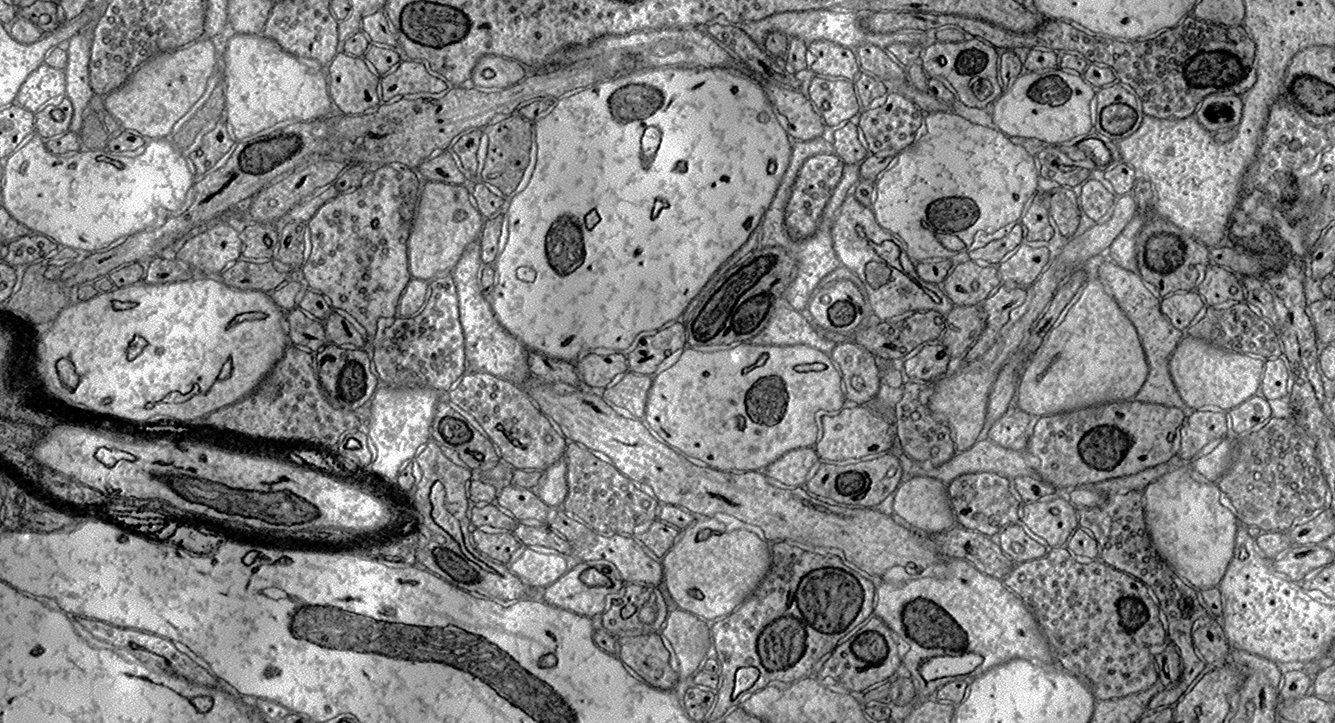
\includegraphics[width=\linewidth]{figures/schema/teaser-image.png}
			(a)
\includegraphics[width=\linewidth]{figures/schema/teaser-segmentation.png}
		\end{minipage}
		\begin{minipage}{0.2\textwidth}
			(b)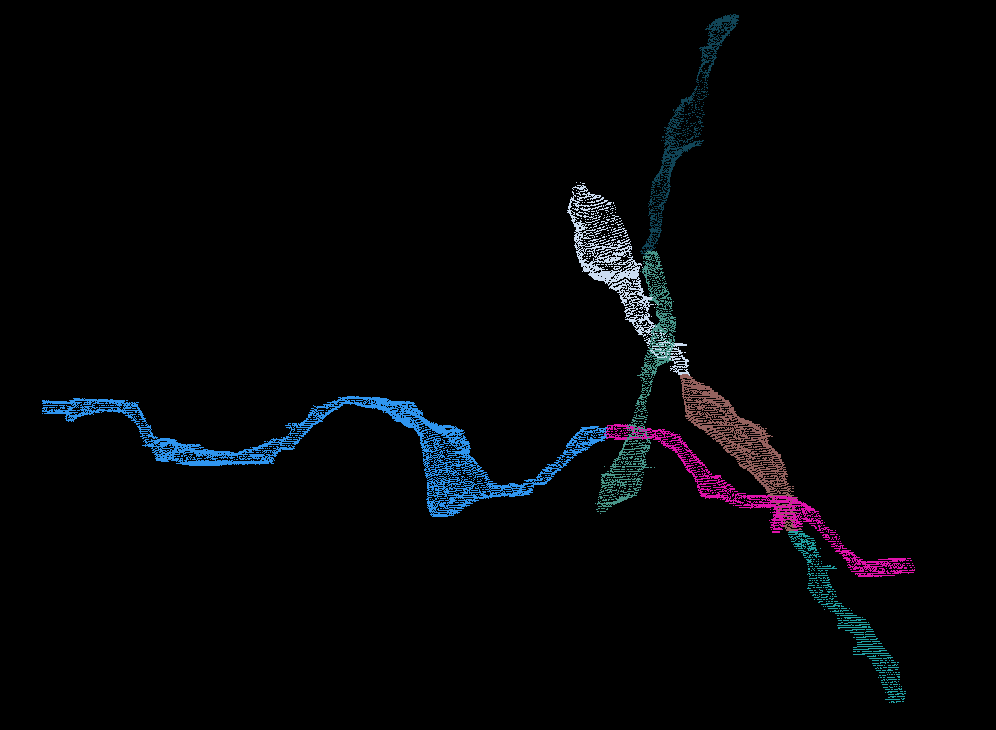
\includegraphics[width=\linewidth]{figures/schema/pre-multicut.png}
		\end{minipage}
		\begin{minipage}{0.3\textwidth}
			(c)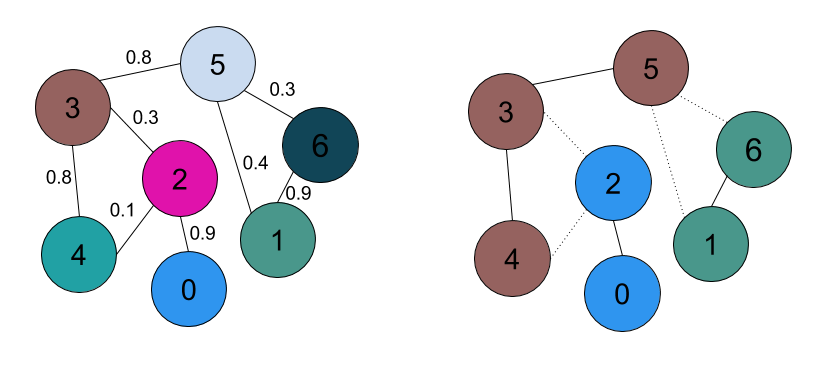
\includegraphics[width=\linewidth]{figures/schema/multicut-graph.png}
		\end{minipage}
		\begin{minipage}{0.2\textwidth}
			(d)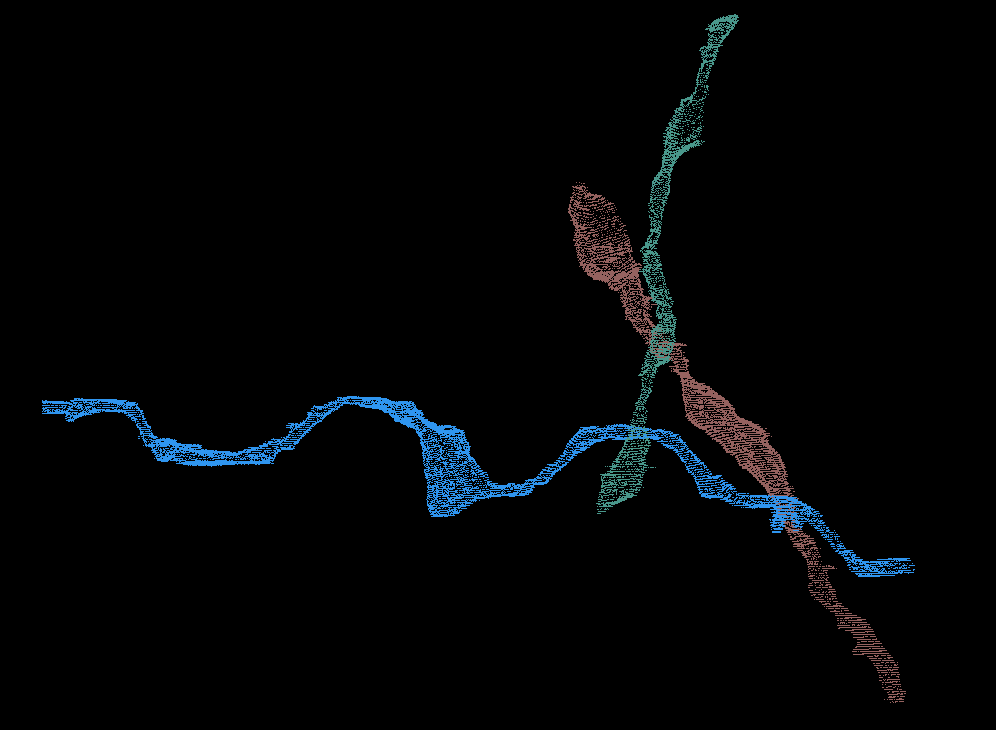
\includegraphics[width=\linewidth]{figures/schema/post-multicut.png}
		\end{minipage}
		\caption{Outline of our approach. (a) Raw EM image data (top) and results of pixel-based segmentation and agglomeration algorithms (bottom). (b) Extracted 3D skeleton from the segmentation. (c) Simplified 3D graph with error probabilities from trained classifier (schematic). (d) Result of graph partitioning algorithm with local and global geometric features (schematic). (d) Improved 3D reconstruction.}
		\label{fig:teaser}
	\end{minipage}
\end{figure}


%%%%%%%%% ABSTRACT
\begin{abstract}
Advancements in electron microscopy image acquisition have created massive connectomics datasets in the terabyte range that make manual reconstruction of neuronal structures infeasible. Current state-of-the-art automatic methods segment neural membranes at the pixel level followed by agglomeration methods to create full neuron reconstructions. However, these approaches widely neglect global geometric properties that are inherent in the graph structure of neural wiring diagrams. Instead, we follow bottom-up pixel-based reconstruction by a top-down graph-based method to more accurately approximate neural pathways. Using the membrane labels of the pixel-based segmentation we first generate skeletons in 3D. Using this 3D graph we train automatic classifiers for shape description to detect impossible neural pathways by looking at geometric properties. We then apply efficient graph-based optimization strategies to improve the segmentation labels. We demonstrate the performance of our approach on multiple real-world connectomics datasets with average variation of information improvement of $X\times$. The paper provides insights into learning shape features for top-down graph-based neuron reconstruction.
\end{abstract}

%%%%%%%%% BODY TEXT
\section{Introduction}

\begin{figure}
	\centering
	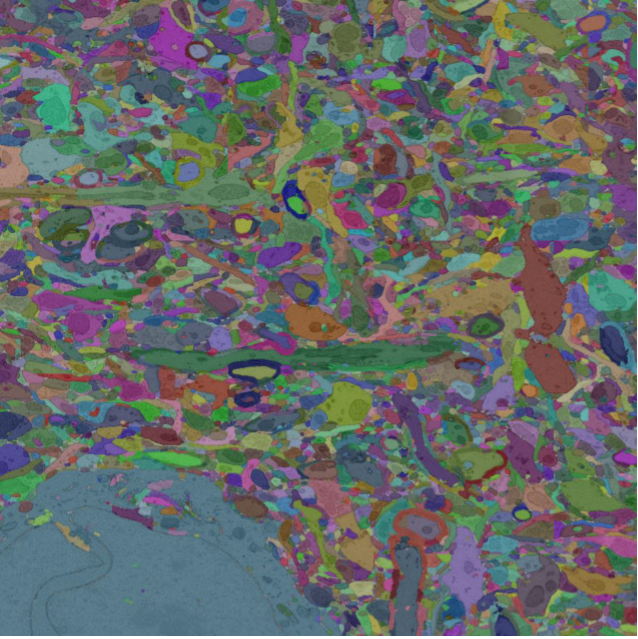
\includegraphics[width=0.42\linewidth]{./figures/intro-slice.png}
	\hspace{0.085\linewidth}
	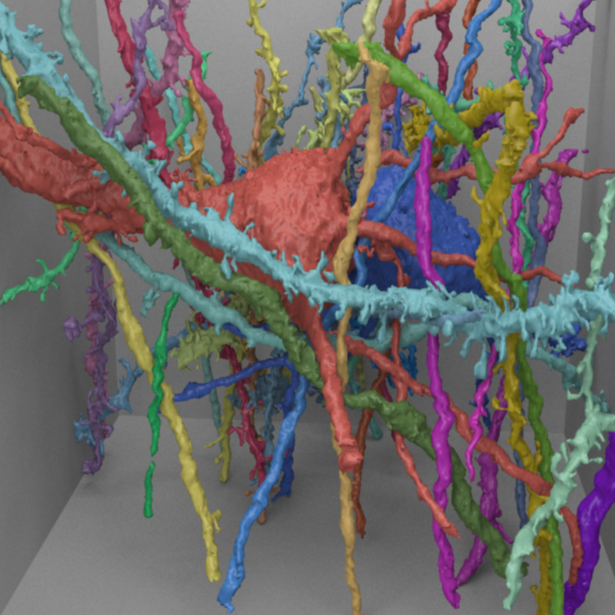
\includegraphics[width=0.42\linewidth]{./figures/intro-cube.png}
\end{figure}

Connectomics, the field of large-scale nanometer reconstruction of the wiring diagram of the brain, has created datasets petabytes in size. With recent advancements in image acquisition, neuroscientists are producing a terabyte of raw electron micronscopy image data every hour \cite{hildebrand2017whole}. Needless to say, it is impossible for domain experts to manually label this bulk of 3-D image data. However, many neuroscientists believe that they will be able to explore new insights into the workings of the brain by creating a complete wiring diagram of the brain \cite{kasthuri2015saturated}. These observations will create new advancements in neuromedicine, artificial intelligence, and (CITE). 

The access to significant datasets and potential for significant scientific contributions to the field of medicine has created a ripe environment for automatic reconstruction of these EM images. Significant research in the field has focused on extracting complete neuron reconstructions using the raw EM images. These techniques use only the image values acquired from the microscopes to agglomerate pixels into neuron predictions. Frequently, convolutional neural networks predict affinities between pixels \cite{ronneberger2015u,lee2015recursive}. 

Using only pixel data is not enough for full reconstruction of these datasets (CITE), and so researchers create a level of abstraction on top of the per-pixel algorithms. Under the new domain, researchers used these per-pixel algorithms as input to agglomerate pixels into super-pixels and create larger neuron reconstructions \cite{nunez2014graph} (CITE NEUROPROOF). These algorithms considered higher level information such as the boundary statistics between pixel regions and simple shape descriptors (CITE LASH).  These algorithms outperform the per-pixel methods from before but still do not fully leverage the wealth of information available.

Here we present another level of abstraction above the agglomeration strategies of the last few years. Our algorithms focus on the overarching shapes of the an oversegmented label volume to determine potential merge candidates. After identifying merge regions, we present a 3-D convolutional neural network to predict merges using only as input the shapes of the regions considered. Lastly, we build all of these techniques into a graph representation of the label volume. This enables us to enforce global constraints on the resulting segmentation that more closely match the biological principles. 

% !TEX root =  paper.tex
\section{Related Work}

A significant amount of research in computer vision focuses on the segmentation of images~\cite{zaitoun2015survey}. Here, we review some of the most successful methods that have been applied to large-scale EM images in connectomics. Fig.~\ref{fig:pipeline} shows the results of a typical connectomics segmentation pipeline.

\paragraph{Pixel-based methods.}
A large amount of connectomics research considers the problem of extracting segmentation information at the pixel (i.e., voxel) level from the raw EM images. Some early techniques apply computationally expensive graph partitioning algorithms with a single node per pixel~\cite{andres2012globally}. However these methods do not scale to terabyte datasets. More recent methods train classifiers to predict membrane probabilities per image slice either using 2D~\cite{ciresan2012deep,jain2010boundary,kaynig2015large,seymour2016rhoananet,amelio_segmentation} or 3D CNNs~\cite{lee2015recursive,ronneberger2015u,turaga2010convolutional}.

Oftentimes these networks produce probabilities for the affinity between two voxels (i.e., the probability that adjacent voxels belong to the same neuron). The MALIS cost function is specifically designed for generating affinities that produce good segmentations~\cite{briggman2009maximin}. More recently, flood-filling networks produce segmentations by training an end-to-end neural network that goes from EM images directly to label volumes~\cite{januszewski2016flood}. These networks produce impressive accuracies but at a high computational cost.

\paragraph{Region-based methods.}
%Lately, many recent advancements in segmentation use artificial neural networks since machine-learned features outperform hand-designed ones~\cite{bogovic2013learned}.
%A significant amount of research focuses on the training and optimization of these deep neural networks~\cite{chatfield2014return,maas2013rectifier,nesterov1983method}.
Several pixel-based approaches generate probabilities that neighboring pixels belong to the same neuron.
Often a watershed algorithm will cluster pixels into small super-pixels~\cite{zlateski2015image}.
Many methods build on top of these strategies and train random-forest classifiers to produce region-based (i.e., super-pixel) segmentations~\cite{seymour2016rhoananet,nunez2014graph,10.1371/journal.pone.0125825,parag2017anisotropic,zlateski2015image}.

\paragraph{Segment-based methods.}
Some recent research builds on top of these region-based methods to correct errors in the segmentation~\cite{rolnick2017morphological,error_correction_using_CNN,haehn2017guided}.
However, to our knowledge, our method is the first to extract a 3D graph from pixel-based agglomerated segmentations for a true top-down reconstruction approach. This allows us to enforce domain-specific constraints using graph-based partitioning algorithms. Many segmentation and clustering algorithms use graph partitioning techniques~\cite{andres2012globally} or normalized cuts for traditional image segmentation~\cite{kappes2016higher,shi2000normalized,tatiraju2008image}.
Even though graph partitioning is an NP-Hard problem~\cite{demaine2006correlation} there are several useful multicut heuristics that provide good approximations with reasonable computational costs~\cite{horvnakova2017analysis}. We use the method of Keuper et al. to partition the extracted 3D graph into the final neuron reconstruction~\cite{keuper2015efficient}.


% !TEX root =  paper.tex
\section{Method}

\begin{figure*}[htbp]
	\begin{center}
		\subfloat[]{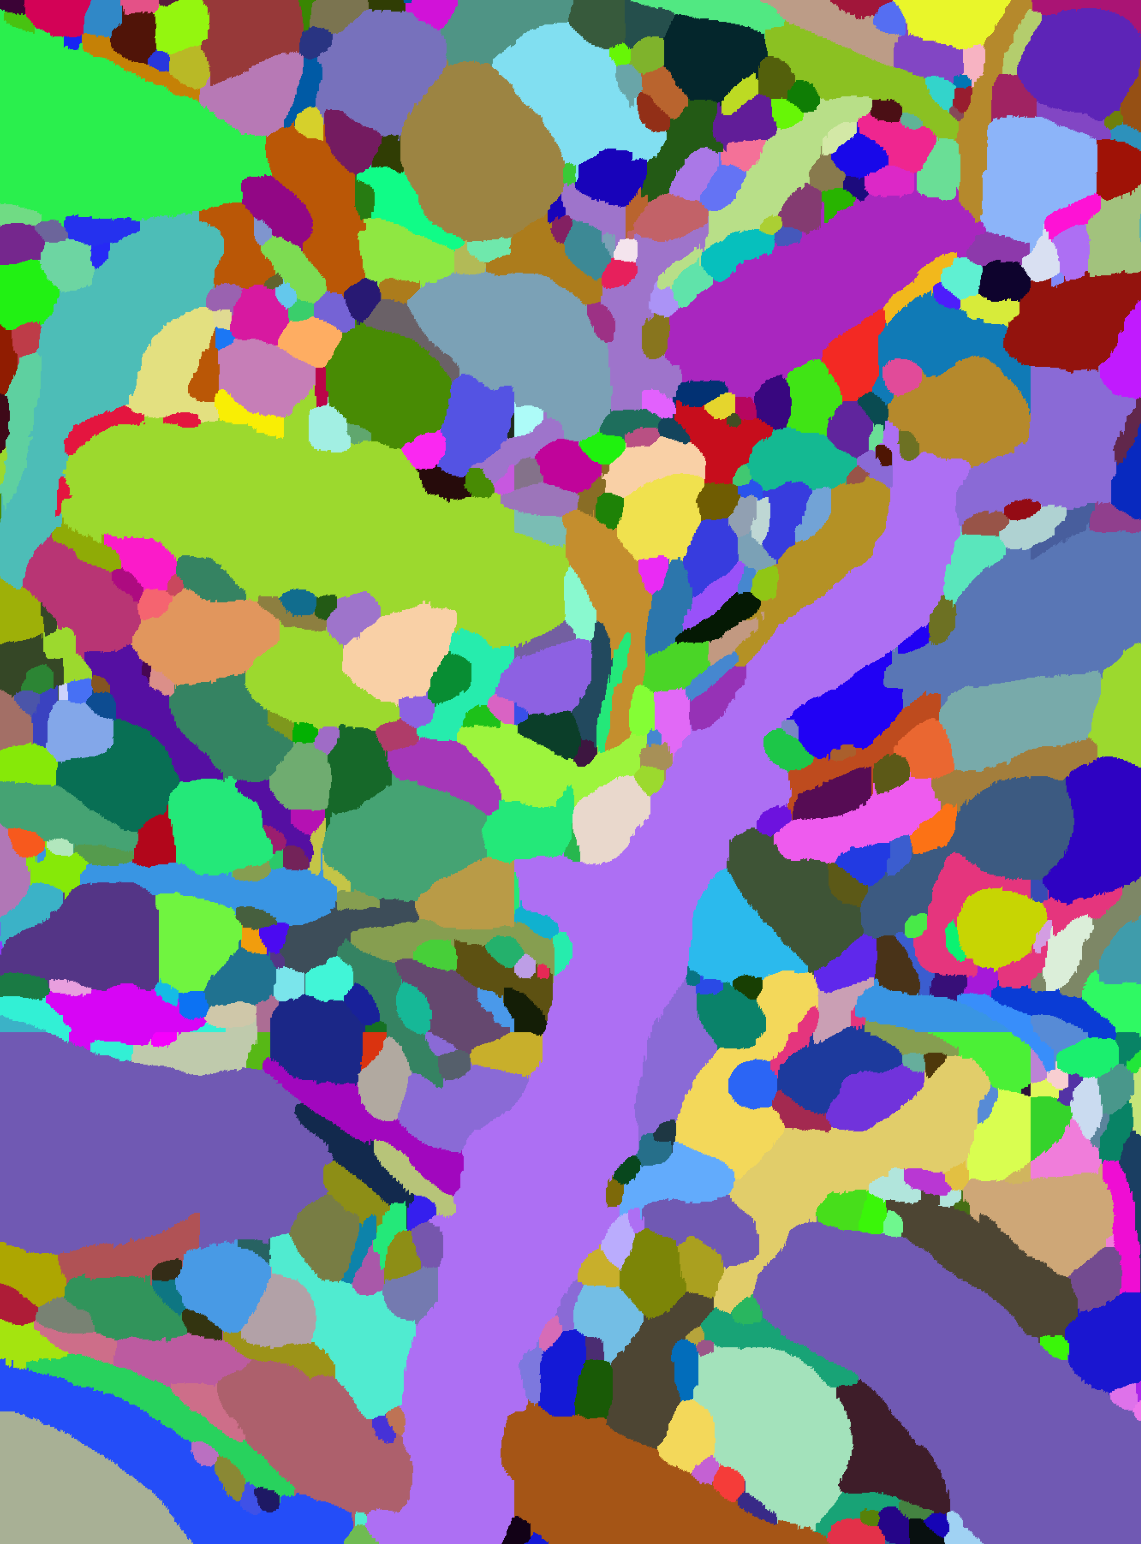
\includegraphics[width=0.24\linewidth]{./figures/methods/multicut_input.png}}
		\subfloat[]{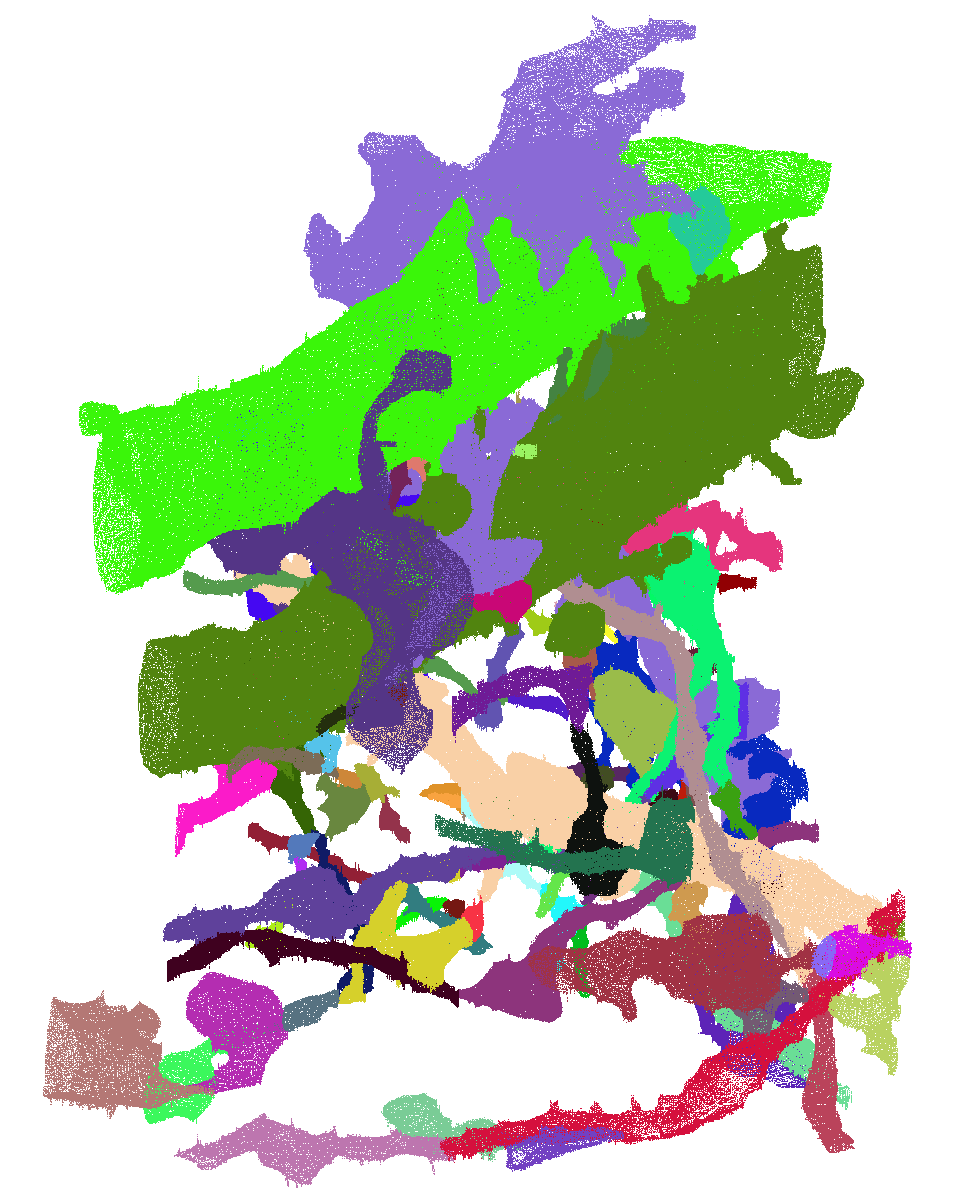
\includegraphics[width=0.24\linewidth]{./figures/methods/pre-multicut.png}}
		\subfloat[]{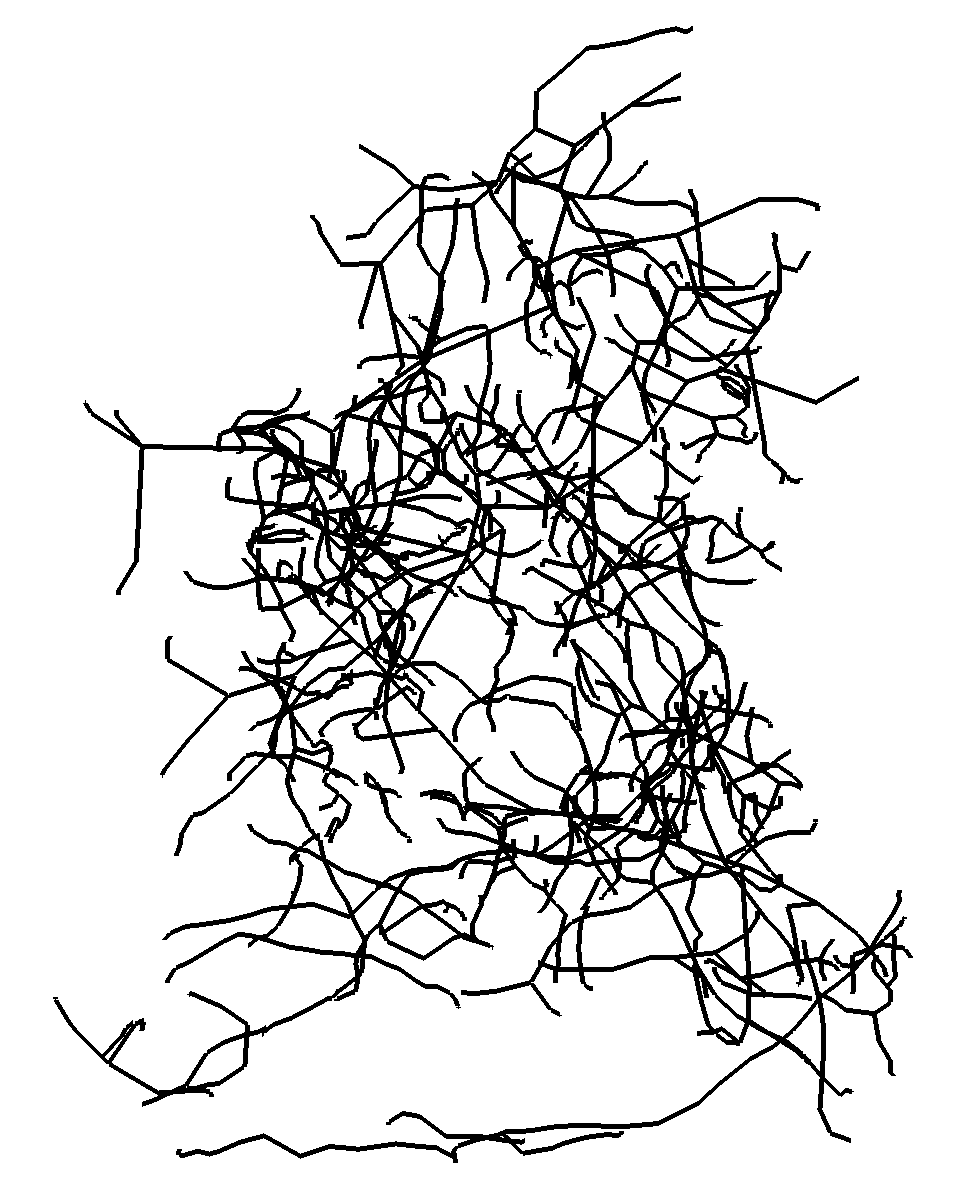
\includegraphics[width=0.24\linewidth]{./figures/methods/multicut-graph.png}}
		\subfloat[]{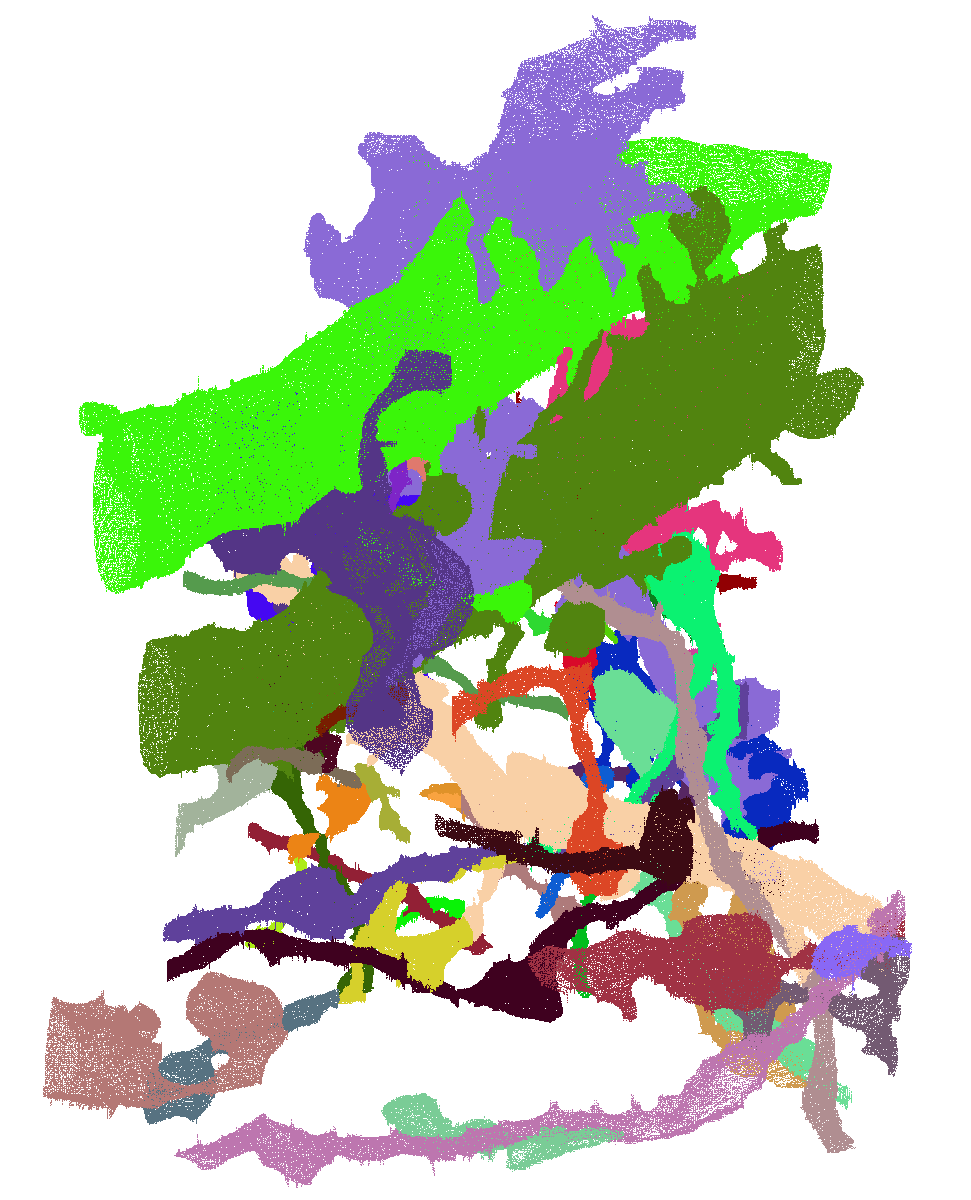
\includegraphics[width=0.24\linewidth]{./figures/methods/post-multicut.png}}
	\end{center}
	\caption{Outline of our approach, from left to right: result of the pixel-based segmentation and agglomeration algorithm; segments of several neurons from the initial segmentation; extracted skeletonized network of those segments; improved 3D reconstruction of the selected segments after graph construction and partitioning with constraints.}
	\label{fig:overview}
\end{figure*}

There are two types of errors that can occur in connectomics segmentations: \textit{split errors} and \textit{merge errors}. 
In a split error, two segments should have been merged into one neuronal process. 
In a merge error, one segment corresponds to more than one neuron.
Generally, it is much more difficult to correct merge errors than to correct split errors,
as the space of possible split proposals grows quickly~\cite{parag2015properties}.
Thus, most reconstruction approaches are tuned towards over-segmentation with many more split than merge errors. 
Our method takes as input over-segmentations of EM image volumes generated by scalable, state-of-the-art connectomics reconstruction pipelines (Sec.~\ref{sec:neuroproof}). 
Our goal is to identify locations of split errors and merge the corresponding segments automatically.

From the input segmentation we generate a graph $G$ with nodes $N$ and edges $E$ with weights $w_e$. 
The nodes correspond to labeled segments from the segmentation.
There are edges between all nodes that we consider as merge candidates.
Ideally, our graph has edges corresponding to all of the segments that were erroneously split. 
To compute this graph we generate a skeleton for every segment in the pixel-based segmentation (Fig.~\ref{fig:overview}). 
The skeletonized 3D network is a simplified representation of the overall branching structure of the neurons. 
From these skeletons we identify potential merge locations and produce the corresponding edges for the graph. 
To find actual merges we run a classification CNN to generate edge weights corresponding to merge probabilities.
We formulate our graph partitioning problem as a multicut problem to segment the nodes into correct neuronal processes. 
We will now discuss the three major components to our framework (graph creation, edge weight assignment, and graph partitioning) in more detail.

\subsection{Node Generation}
%\subsubsection{Node Generation}
\label{sec:skeletonization}

The simplest node generation strategy creates one node for every unique segment label in the input volume. 
However, some of the labels in the volume correspond to very small structures that are likely the result of segmentation errors, typically in regions with noisy raw image data. 
It is difficult to extract useful shape features from these segments because of their small, often random, shape. 
We prune these nodes from the graph by removing all segments with fewer than a threshold $t_{seg} = 20,000$ voxels. 
This removes on average \TODO{XX}\% of the segments in our  datasets (Sec.~\ref{sec:dataset}), leaving us with around $\TODO{XX}$ nodes per dataset (\TODO{X nodes per micrometer}). 
Despite the large number of segments, these regions only take up \TODO{XX}\% of the total volume on average.
We provide further analysis of this strategy in the supplemental material. 

\subsection{Edge Generation}

\begin{figure}[t]
	\centering
	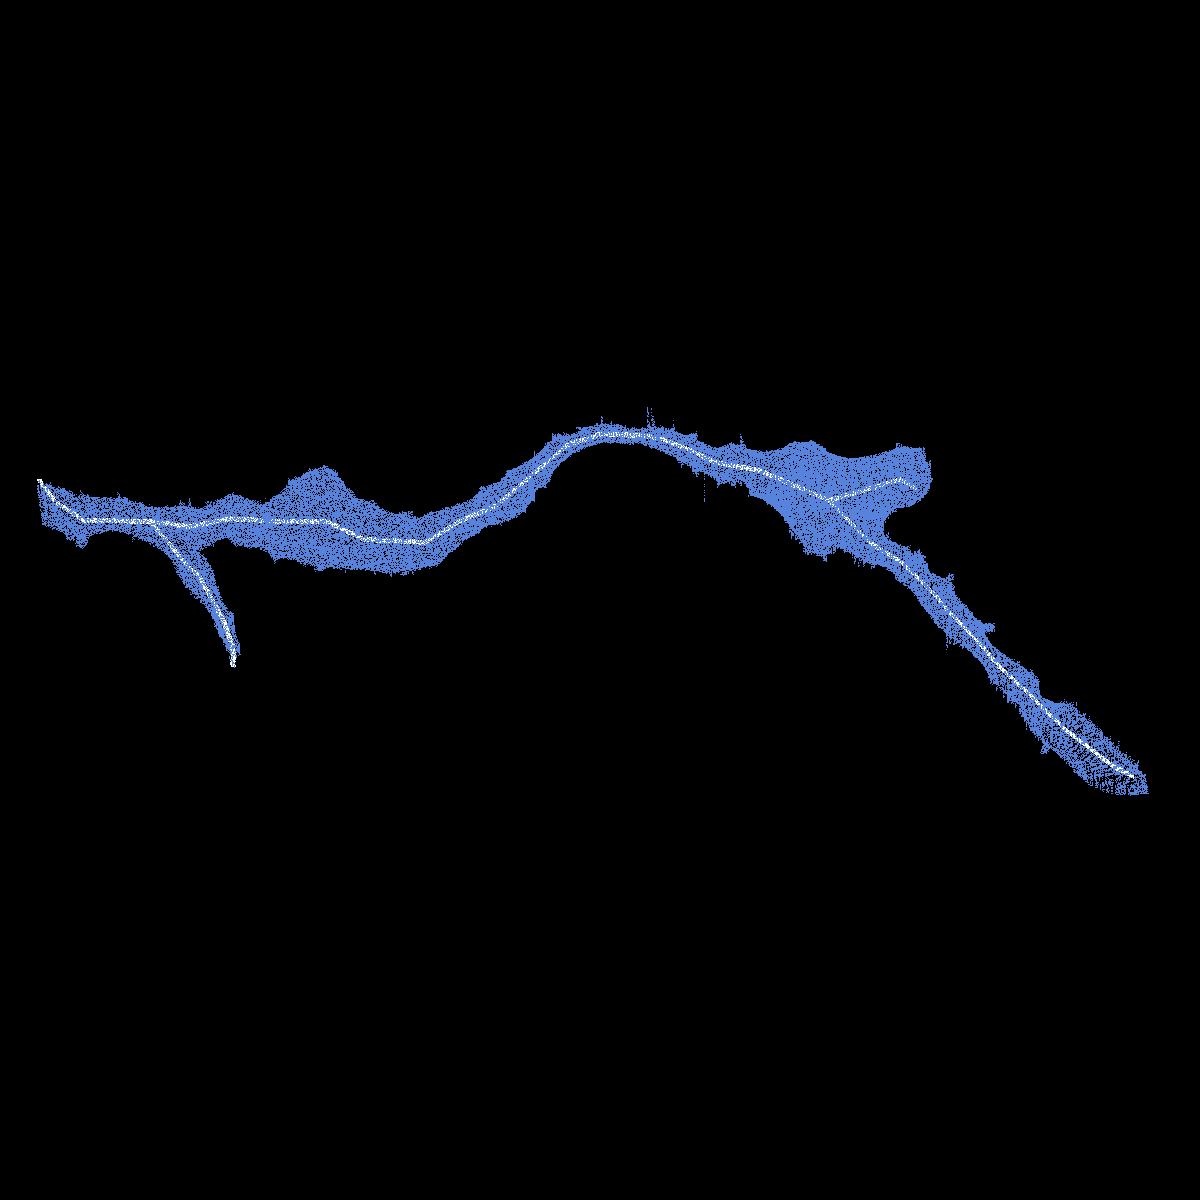
\includegraphics[width=0.45\linewidth]{./figures/skeleton1.png}
	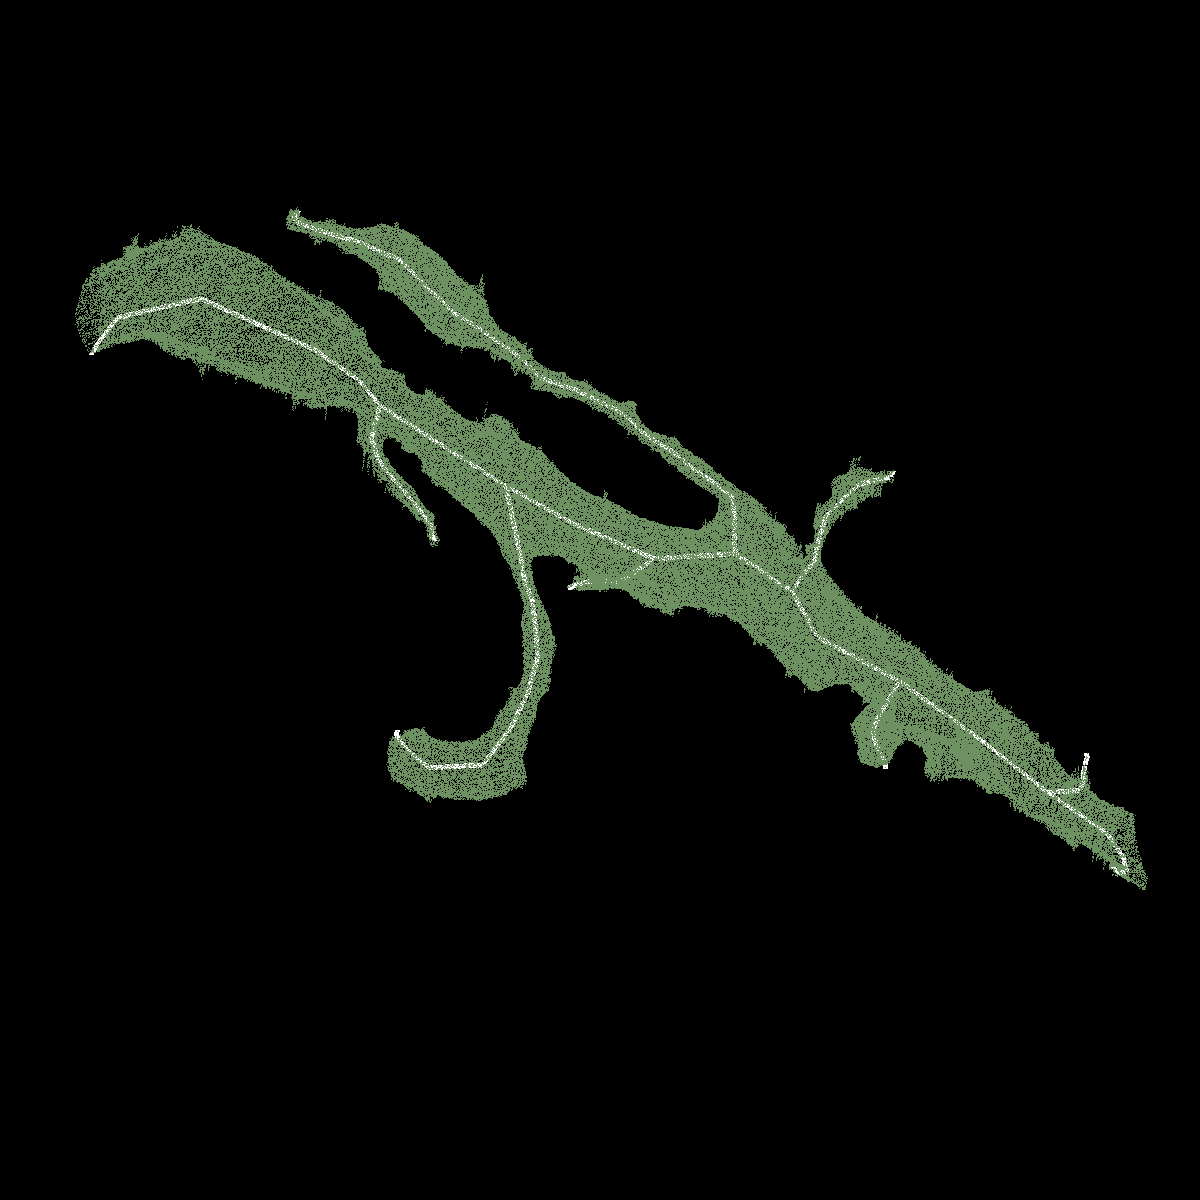
\includegraphics[width=0.45\linewidth]{./figures/skeleton2.png}
	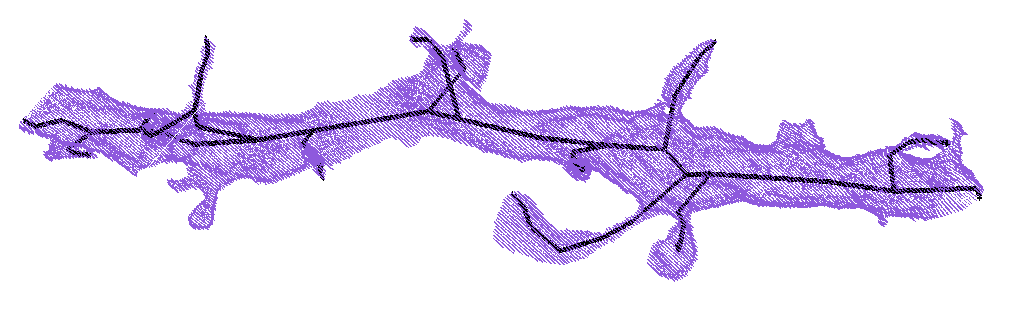
\includegraphics[width=0.45\linewidth]{./figures/skeleton3.png}
	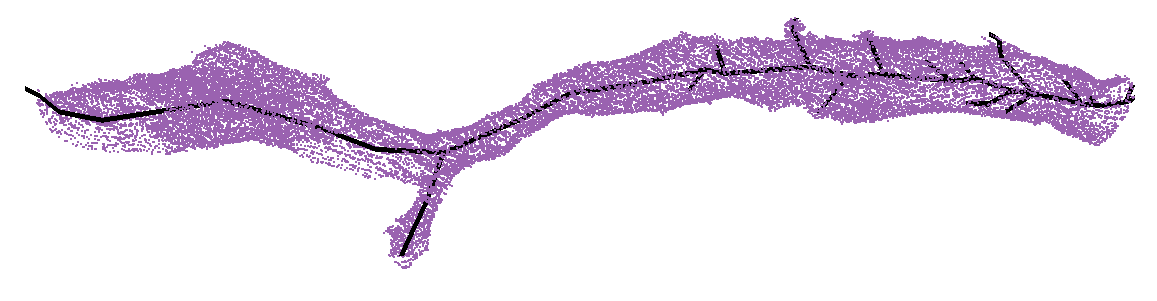
\includegraphics[width=0.45\linewidth]{./figures/skeleton4.png}
	\caption{Example skeletons (in black) extracted from segments using a variant of the TEASER algorithm.}
	\label{fig:skeletonization}
\end{figure}

A typical approach for generating edges produces one between all adjacent segments. Two segments $l_1$ and $l_2$ are considered adjacent if there is a pair of adjacent voxels with one labeled $l_1$ and the other labeled $l_2$.
For example, pixel-based agglomeration methods such as mean agglomeration \TODO{CITE} or waterz \TODO{CITE} consider all pairs of adjacent segments for merging.
However, this method produces too many edges in the graph for graph-based optimization approaches. 
We identify a smaller number of pairs of segments to consider as graph edges using the following approach.

First, we extract a skeleton from each segment in the label volume using a variant~\cite{zhao2014automatic} of the TEASER algorithm~\cite{sato2000teasar}. 
This skeletonization algorithm repeatedly uses Dijkstra's algorithm to find the farthest voxel from a seed location. 
Since this algorithm is non-linear in the number of voxels, we downsample the datasets so that there are voxel samples every $\SI{30}{\nano\meter}$ in each dimension.
Empirically, this reduced the running time for skeletonization by $\TODO{XX\%}$, with minimal reduction in skeleton accuracy ($\TODO{XX\%}$ fewer branches). 
Fig.~\ref{fig:skeletonization} shows three examples of extracted skeletons (in black). 
These skeletons consist of a sequence of \textit{joints}, i.e., locations that are locally a maximum distance from the segment boundary, with line segments connecting successive joints. 
We prune the joints that are within $t_{jnt} = \TODO{XX}\SI{}{\nano\meter}$ of each other to reduce unnecessary branching.
This value is small enough that the skeletons extend into the spines but large enough to keep branching does to a reasonable level.
Additional analysis is available in the supplemental material.
We refer to joints that have only one connected neighbor as \textit{endpoints}. 
We find that approximately \TODO{XX\%} of the segments that are erroneously split have nearby endpoints  (Fig.~\ref{fig:merge_candidates}). 
We make use of this fact to find merge candidates with the following two-pass pruning algorithm.

In the first pass, we iterate over all endpoints $e$ belonging to a segment $S$ and create a set of segments $\mathbb{S}_e^\prime$ that includes all labels that are within $t_{low}$ voxels from $e$.
Elements of $\mathbb{S}_e^\prime$ are candidates for merging. 
However, this first pass often leads to too many candidates, requiring an additional pass for further pruning. 
In the second pass, we consider all of the segments in $\mathbb{S}_e^\prime$ for every endpoint $e$. 
If a segment $S^\prime \in \mathbb{S}_e^\prime$ has an endpoint within $t_{high}$ voxels of $e$, the segment $S$ and $S^\prime$ are considered for merging. 
We store the midpoints between the two endpoints as the center of the potential merge in the set $\mathbb{S}_c$. 
This algorithm produces a set of segments to consider for merging. Only these pairs have a corresponding edge in the constructed graph.

\subsection{Edge Weights Assignment}
\label{sec:edge-weights}
We assign edge weights $w_e$ to each edge where the weight corresponds to the probability that two nodes belong to the same neuron.
We train a 3D CNN classifier to learn from the manually labeled oversegmentation input volume (Sec.~\ref{sec:dataset}).
If the probability that the nodes belong to the same neuron is $p_e$, the edge weight $w_e = \log{\frac{p_e}{1 - p_e}} + \log{\frac{1 - \beta}{\beta}}$, where $\beta$ is a tunable parameter that encourages over- or under-segmentation.

\subsubsection{Classifier Input}

We extract a cubic region of interest (ROI) around each endpoint $e$ in $\mathbb{S}_c$ as input to the CNN. 
The CNN receives three input channels for every voxel in the ROI around segments $l_1$ and $l_2$. 
The input in all of the channels is in the range $\{-0.5, 0.5\}$. 
The first channel is $0.5$ only if the corresponding voxel has label $l_1$. 
The second channel is $0.5$ only if the corresponding voxel has label $l_2$. 
The third channel is $0.5$ if the corresponding voxel is either $l_1$ or $l_2$.
We do not use the raw EM image information to avoid the need to retrain the network on datasets that have been stained differently or imaged at different resolution. 
This reduces the need for generating costly manually-labeled ground truth. 

\begin{figure}[t]
	\centering
	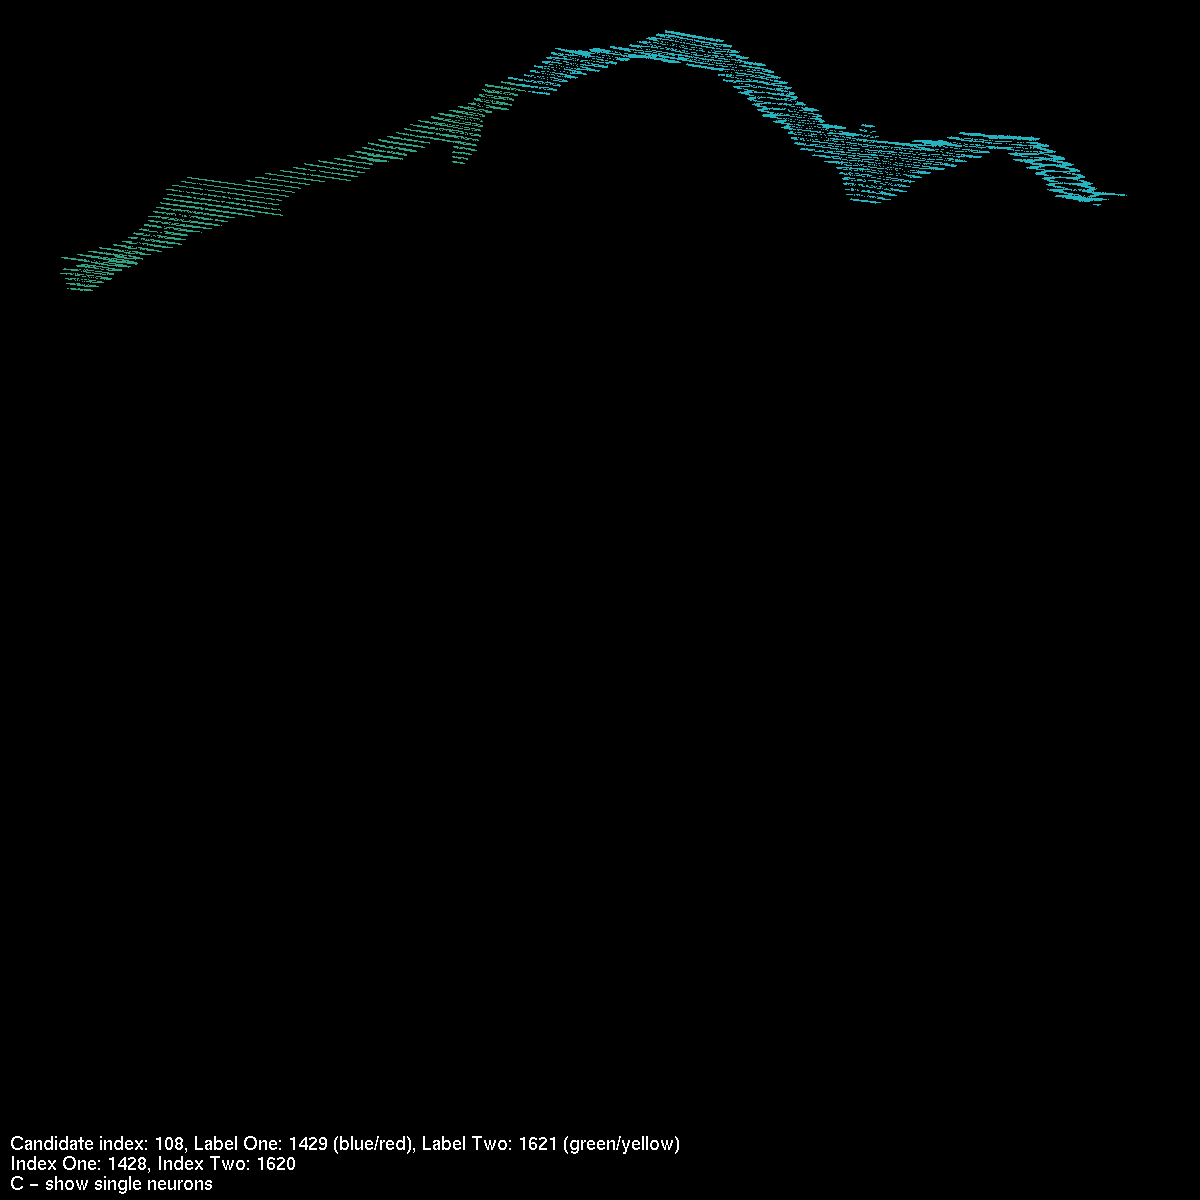
\includegraphics[width=0.32\linewidth]{./figures/split_error1.png}
	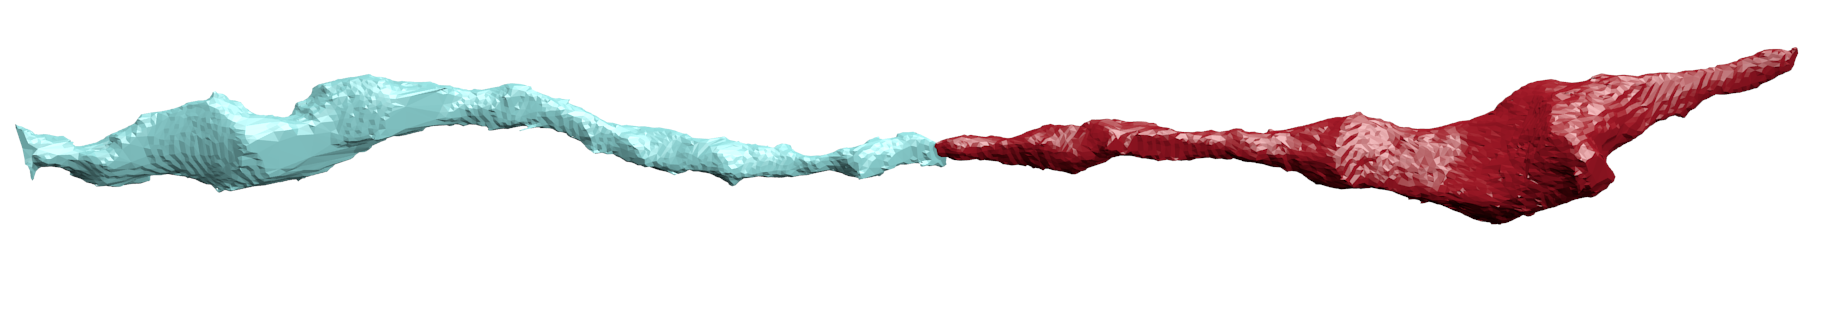
\includegraphics[width=0.32\linewidth]{./figures/split_error2.png}		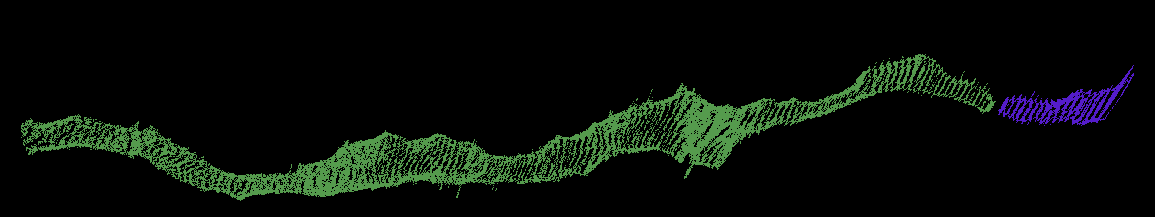
\includegraphics[width=0.32\linewidth]{./figures/merge_candidate2.png}
	\caption{Three erroneously split segments.}
	\label{fig:merge_candidates}
\end{figure}

\subsubsection{Network Architecture \& Training}

We use \textit{VGG-style} blocks as presented by Chatfield et al.~\cite{chatfield2014return}. 
Each blocks consists of two double convolutions with filter size $3\times3\times3$ followed by a max pooling step. 
There are three layers of these blocks. 
The first two max pooling layers are anisotropic with pooling only in the $x$ and $y$ dimensions. 
The output of this final pooling step is flattened into a 1D vector that is input into two fully connected layers. 
The final layer produces probabilities with a sigmoid activation function~\cite{funahashi1989approximate}. 
All of the other activation functions are LeakyReLU~\cite{maas2013rectifier}.

For training we use a stochastic gradient descent optimizer with Nesterov's accelerated gradient~\cite{nesterov1983method}. 
We employ dropouts of $0.2$ after every pooling layer and the first dense layer, and a dropout of $0.5$ after the final dense layer to prevent overfitting. 
We discuss all other network parameters in Sec.~\ref{sec:network-parameters}.

\subsection{Graph Clustering}

After constructing the 3D graph we seek to partition the graph into labels where every label corresponds to a neuronal process. 
We formulate this graph partitioning problem as a multicut problem.
There are two primary benefits to using a multicut formulation. 
First, the number of segments in the final graph is not predetermined but depends on the input graph itself. 
Second, this minimization produces globally consistent solutions (i.e. a boundary remains if and only if the two corresponding nodes belong to unique segments).

We apply the algorithms of Keuper et al.~\cite{keuper2015efficient} to produce a feasible solution to the multicut problem using greedy additive edge contraction.
Following their example, we employ the generalized ``lifted'' multicut formulation.
Traditional multicut solutions only consider the probabilities that two adjacent nodes belong to the same segment. 
In the ``lifted'' extension to the problem, we can penalize non-adjacent nodes that belong to different segments. 
These penalties between non-adjacent nodes are called ``lifted'' edges. 
Ideally these ``lifted'' weights represent the probability that two nodes belong to the same neuron given all such possible paths in the graph between the nodes.
However, determining such probabilities is computationally expensive.
We approximate these probabilities by finding the maximal probable path between any two nodes using Dijkstra's algorithm~\cite{keuper2015efficient}.
Since our graphs are sufficiently small, we can generate ``lifted'' edges between all pairs of nodes. 

\paragraph{Post-processing}

By reformulating the segmentation problem as a graph partitioning one, we can enforce some global constraints on our result based on the underlying biology.
Traditional hierarchical clustering algorithms do not rely on such constraints but consider local decisions independently.
We enforce a global constraint that neurons are tree-structured and should not contain cycles. 
The multicut problems returns a series of ``collapsed'' edges between nodes that belong to the same neuron.
We iterate over these edges in order of the probability of merge generated by our CNN. 
We ``collapse'' an edge only if it does not create a cycle in the graph.


% !TEX root =  paper.tex
\section{Experiments}

We evaluate our method by comparing it to a state-of-the-art pixel-based reconstruction approach using datasets from mouse and fly brains.

\subsection{Datasets}
\label{sec:dataset}

Our proposed method is designed for very large connectomics datasets. 
Popular challenge datasets such as CREMI and SNEMI3D are simply too small for any noticeable change. 
The following datasets contain 4 times more volume than the CREMI datasets. \TODO{better to have a table here}
\\~\\
%\subsubsection{Kasthuri}
\noindent\textbf{Kasthuri}
The Kasthuri dataset consists of scanning electron microscope images of the neocortex of a mouse brain~\cite{kasthuri2015saturated}. 
This dataset is $5342 \times 3618 \times 338$ voxels in size. 
The resolution of the dataset is $\SI[product-units=single]{3 x 3 x 30}{\nano\meter}^3$ per voxel. 
We evaluate our methods using the left cylinder of this 3-cylinder dataset. 
We downsample the dataset in the $x$ and $y$ dimensions to give a final resolution of $\SI[product-units=single]{6 x 6 x 30}{\nano\meter}^3$ per voxel. 
We divide the dataset into two volumes (Vol. 1 and Vol. 2) along the $x$ dimension, where each volume is $\SI[product-units=single]{8.0 x 10.9 x 10.1}{\micro\meter}^3$ or $1335 \times 1809 \times 338$ voxels.
\\~\\
%\subsubsection{FlyEM}
\noindent\textbf{FlyEM}
The FlyEM dataset comes from the mushroom body of a 5-day old adult male \textit{Drosophila} fly imaged by a focused ion-beam milling scanning electron microscopy~\cite{takemura2017connectome}.
The mushroom body in this species is the primary site of associative learning. 
The original dataset contains a $\SI[product-units=single]{40 x 50 x 120}{\micro\meter}^3$ volume with a resolution of $\SI[product-units=single]{10 x 10 x 10}{\nano\meter}^3$ per voxel. 
We use two cubes (Vol. 1 and Vol. 2) of size $\SI[product-units=single]{10 x 10 x 10}{\micro\meter}^3$ or $999 \times 999 \times 999$ voxels.

%\subsubsection{Fib-25}
%\noindent\textbf{Fib-25}
%The Fib-25 dataset comes from the visual system of a \textit{Drosophila} fly~\cite{takemura2015synaptic}. This sample is %imaged at a resolution of $\SI[product-units=single]{8 x 8 x 8}{\nano\meter}^3$ and has $2588 \times 2108 \times 2876$ %voxels representing a volume of $\SI[product-units=single]{23.0 x 16.9 x 23.0}{\micro\meter}^3$. 
%There is currently a reconstruction challenge based on this sample.

\subsection{Method Configuration}
\noindent\textbf{Initial Segmentation}
%\label{sec:neuroproof}
%The segmentation of the Kasthuri dataset was computed by agglomerating 3D supervoxels produced by the watershed algorithm from 3D affinity predictions~\cite{zlateski2015image}. 
%A recent study by Funke et al.~\cite{funke2017deep} demonstrated superior performance of such methods over existing ones on anisotropic data. 
%We learn 3D affinities using MALIS loss with a U-net~\cite{ronneberger2015u,Turaga:2009}. 
%We apply the z-watershed algorithm with suitable parameters to compute a 3D oversegmentation of the volume. 
%The resulting 3D oversegmentation is then agglomerated using the technique of context-aware delayed agglomeration to generate the final segmentation~\cite{10.1371/journal.pone.0125825}.
For the Kasthuri dataset, we used the segmentation pipeline from Funke et al.~\cite{funke2017deep}. 
We first train a 3D affinity prediction U-Net model~\cite{ronneberger2015u} with MALIS loss~\cite{Turaga:2009} and apply the watershed and agglomeration method~\cite{funke2017deep} to obtain the final segmentation result.
For the FlyEM data, based on the authors' suggestion~\cite{takemura2017connectome}, we apply a context-aware delayed agglomeration algorithm~\cite{10.1371/journal.pone.0125825} that shows improved performance on this dataset over the pipeline used in the original publication. 
This segmentation framework learns voxel and supervoxel classifiers with an emphasis to minimize under-segmentation error. 
The algorithm first computes multi-channel 3-D predictions for membranes, cell interiors, and mitochondria, among other cell features. 
The membrane prediction channel is used to produce an over-segmented volume using 3D watershed, which is then agglomerated hierarchically up to a certain confidence threshold. 
We used exactly the same parameters as the publicly available code for this algorithm.
%For the Fib-25 challenge dataset, we use the segmentation from Funke et al. as our input~\cite{funke2017deep}.
\\~\\
\noindent\textbf{Graph Generation}
The two parameters for the graph pruning algorithm (Sec.~\ref{sec:skeletonization}) are $t_{low}$ and $t_{high}$. 
Ideally, our graph will have an edge for every over-segmented pair of labels with few edges between correctly segmented pairs. 
After considering various thresholds, we find that $t_{low} = \SI{210}{\nano\meter}$ and $t_{high} = \SI{300}{\nano\meter}$ produce expressive graphs with a scalable number of nodes and edges.
We explore these thresholds in greater detail in the supplemental material.
During implementation, we use nanometers instead of voxels for these thresholds to have uniform units across all datasets.
% Connectomics datasets often have lower sample resolutions in $z$ because of limitations during sample preparation. 
% Using nanometers allows us to have uniform units across all of these datasets and calculate the thresholds in voxels at runtime.
% Although the voxels vary between different datasets, the physical space remains constant. 
\\~\\
\noindent\textbf{Edge Weight Learning}
\label{sec:network-parameters}
We use half of the Kasthuri dataset for training and validation. 
We train on 80\% of the potential merge candidates for this volume.
We validate the CNN classifier on the remaining 20\% of the candidates. 
Since our input does not require the image data, we can train on the anisotropic Kasthuri data and test on the isotropic FlyEM data.

We consider networks with varying input sizes, optimizers, loss functions, filter sizes, learning rates, and activation functions. 
The supplemental material includes information on the experiments that determined these final parameters. 
We provide all parameters of the final network in the supplemental material. 
There are 2,313,969 learnable parameters in our final architecture. 
All the parameters are randomly initialized following the Xavier uniform distribution~\cite{glorot2010understanding}. 
Training concluded after 1000 epochs.

%\noindent\textbf{Training Augmentation.}
Since our input is an existing segmentation of the EM images, there are very few training examples compared to per-pixel classifiers that can train on a unique window for each voxel. 
The Kasthuri dataset represents a region of brain over $\SI[product-units=single]{800}{\micro\meter}^3$ in volume and only yields 640 positive merge examples and 4821 negative ones.
To avoid overfitting our deep networks, we apply the following augmentations on the training examples.
During a single batch, we randomly select ten positive and negative examples. 
With probability 0.5, the example is reflected across the $xy$-plane. 
We then rotate the example by a random angle between $0$ and $360$ degrees using nearest neighbor interpolation. 
The supplemental material contains experiments demonstrating the benefits of this augmentation strategy.
We have 20,000 such examples per epoch.
\\~\\
\noindent\textbf{Graph Partition}
%We assign the edges in our graph a weight $w_e = \log{\frac{p_e}{1 - p_e}} + \log{\frac{1 - \beta}{\beta}}$ where $\beta$ is a tunable parameter. 
%Higher values of $\beta$ encourage over-segmentation.
Figure~\ref{fig:variation-of-information} shows our results for variables $\beta \in [0.5, 0.9]$. 
For our multicut analysis we consider $\beta = 0.5$. 

\subsection{Error Metrics}
\label{sec:variation-of-information}
We evaluate the performance of the different methods using the split variation of information (VI)~\cite{meila2003comparing}.
Given a ground truth labeling $GT$ and our automatically reconstructed segmentation $SG$, over- and under-segmentation are quantified by the conditional entropies $H(GT | SG)$ and $H(SG | GT)$, respectively. 
Since we are measuring the entropy between two clusterings, lower VI scores are better.

We use precision and recall to evaluate the convolutional neural network and multicut outputs. 
Since our method attempts to only correct \textit{split errors}, we define a true positive as a pair of segments that are correctly merged together after our pipeline.


% !TEX root =  paper.tex
\section{Results}

\begin{figure*}[t!]
	\centering
	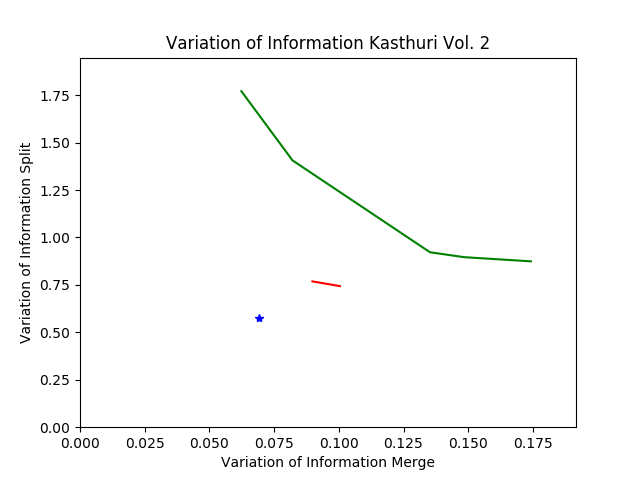
\includegraphics[width=0.32\linewidth]{./figures/variation_of_information-microns-test-600.png}
	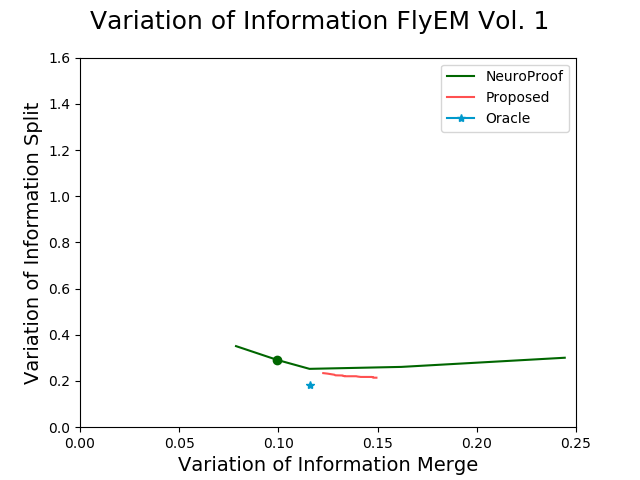
\includegraphics[width=0.32\linewidth]{./figures/variation_of_information-FlyEM-train-600.png}
	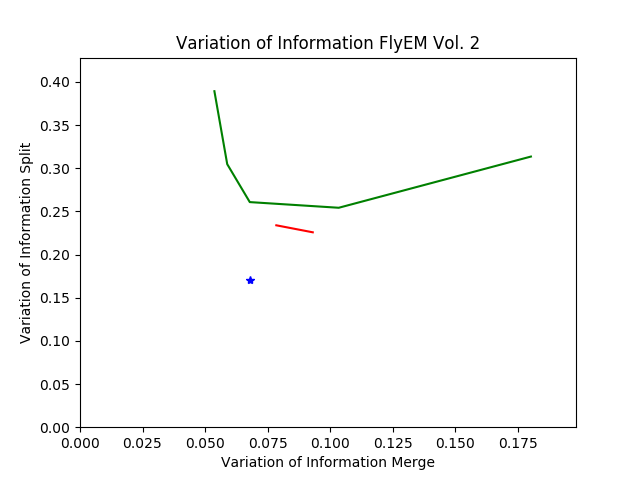
\includegraphics[width=0.32\linewidth]{./figures/variation_of_information-FlyEM-test-600.png}
	\caption{VI scores of our method (red) compared to the baseline segmentation (green) and an oracle (blue) that optimally partitions the graph based on ground truth. Lower scores are better. Our method improves the accuracy of the segmentation in all cases.}
	\label{fig:variation-of-information}
\end{figure*}

\subsection{Variation of Information Results}

In Fig.~\ref{fig:variation-of-information}, we show the VI results of the pixel-based reconstructions of the Kasthuri and FlyEM data (Sec.~\ref{sec:neuroproof}) for varying thresholds of agglomeration (green). 
We use one of these segmentations (green circle) as our input dataset with an agglomeration threshold of 0.3 for all datasets. 
The results from our method are shown in red for varying the $\beta$ parameter. 
We show comparisons to an oracle (blue) that correctly partitions the graph from our method based on ground truth.

Our algorithm improves the accuracy of the reconstruction for every dataset, reducing the VI split score on average by \TODO{XX}\% on the three testing datasets. 
Scores closer to the origin are better for this metric, and in every instance our results are below the green curve.
We see significant improvements on the Kasthuri datasets (VI split reduction of \TODO{XX}\%) and more modest improvements on the FlyEM dataset (reduction of \TODO{XX}\%) and Fib-25 dataset (reduction of \TODO{XX}\%). 

Fig.~\ref{fig:qualitative-results} (left) shows successful merges on the Kasthuri dataset. 
Several of these examples combine multiple consecutive segments that span the volume.
In the third example on the left we correct the over-segmentation of a dendrite and attached spine-necks.
Fig.~\ref{fig:qualitative-results} (right) shows typical failure cases of our method (red circles).
In two of these examples the algorithm correctly predicted several merges before a single error rendered the segment as wrong.
In the third example (blue circle) a merge error in the initial segmentation propagated to our output.
We now analyze how each major component of our method contributes to this final result.

\begin{figure}[t]
	\begin{minipage}{0.45\linewidth}
		\centering
		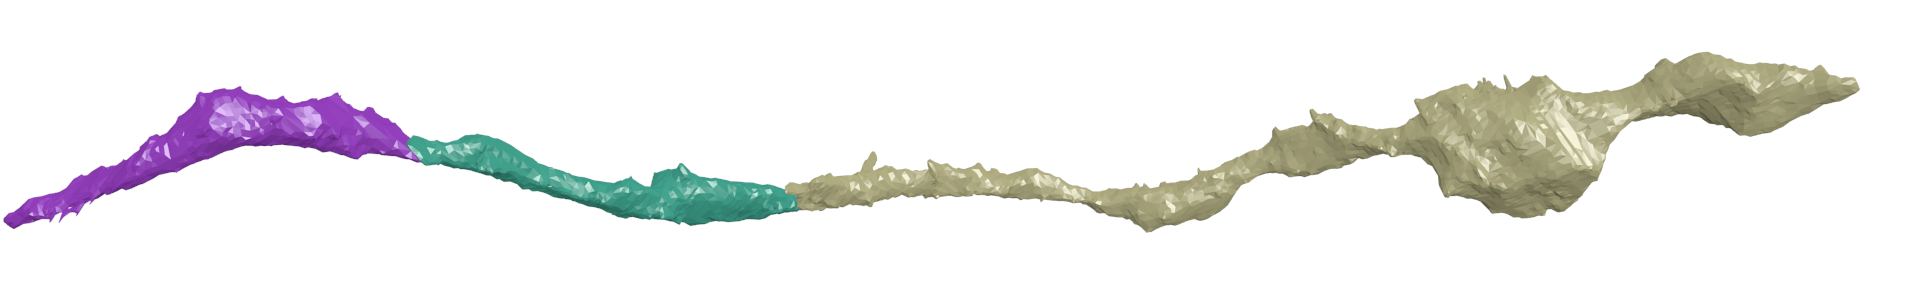
\includegraphics[width=0.85\linewidth]{./figures/VI-results/multicut-correct1.png}
		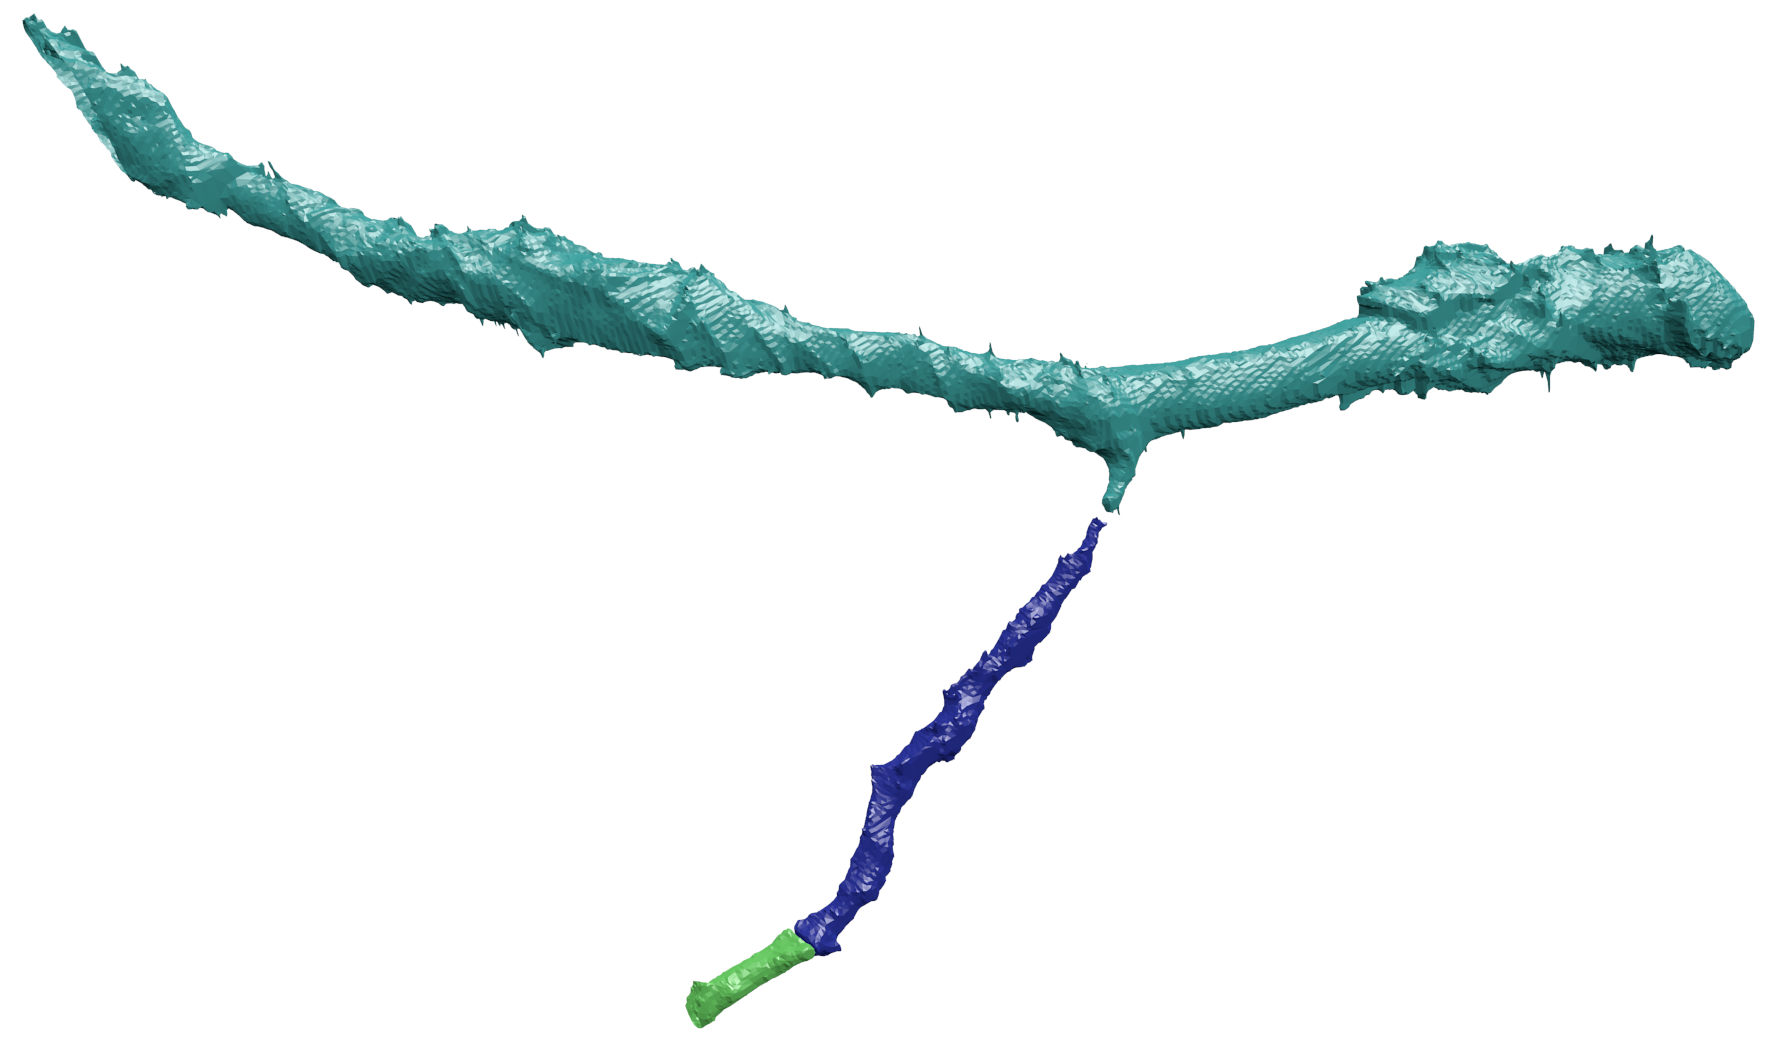
\includegraphics[width=0.85\linewidth]{./figures/VI-results/multicut-correct2.png}
		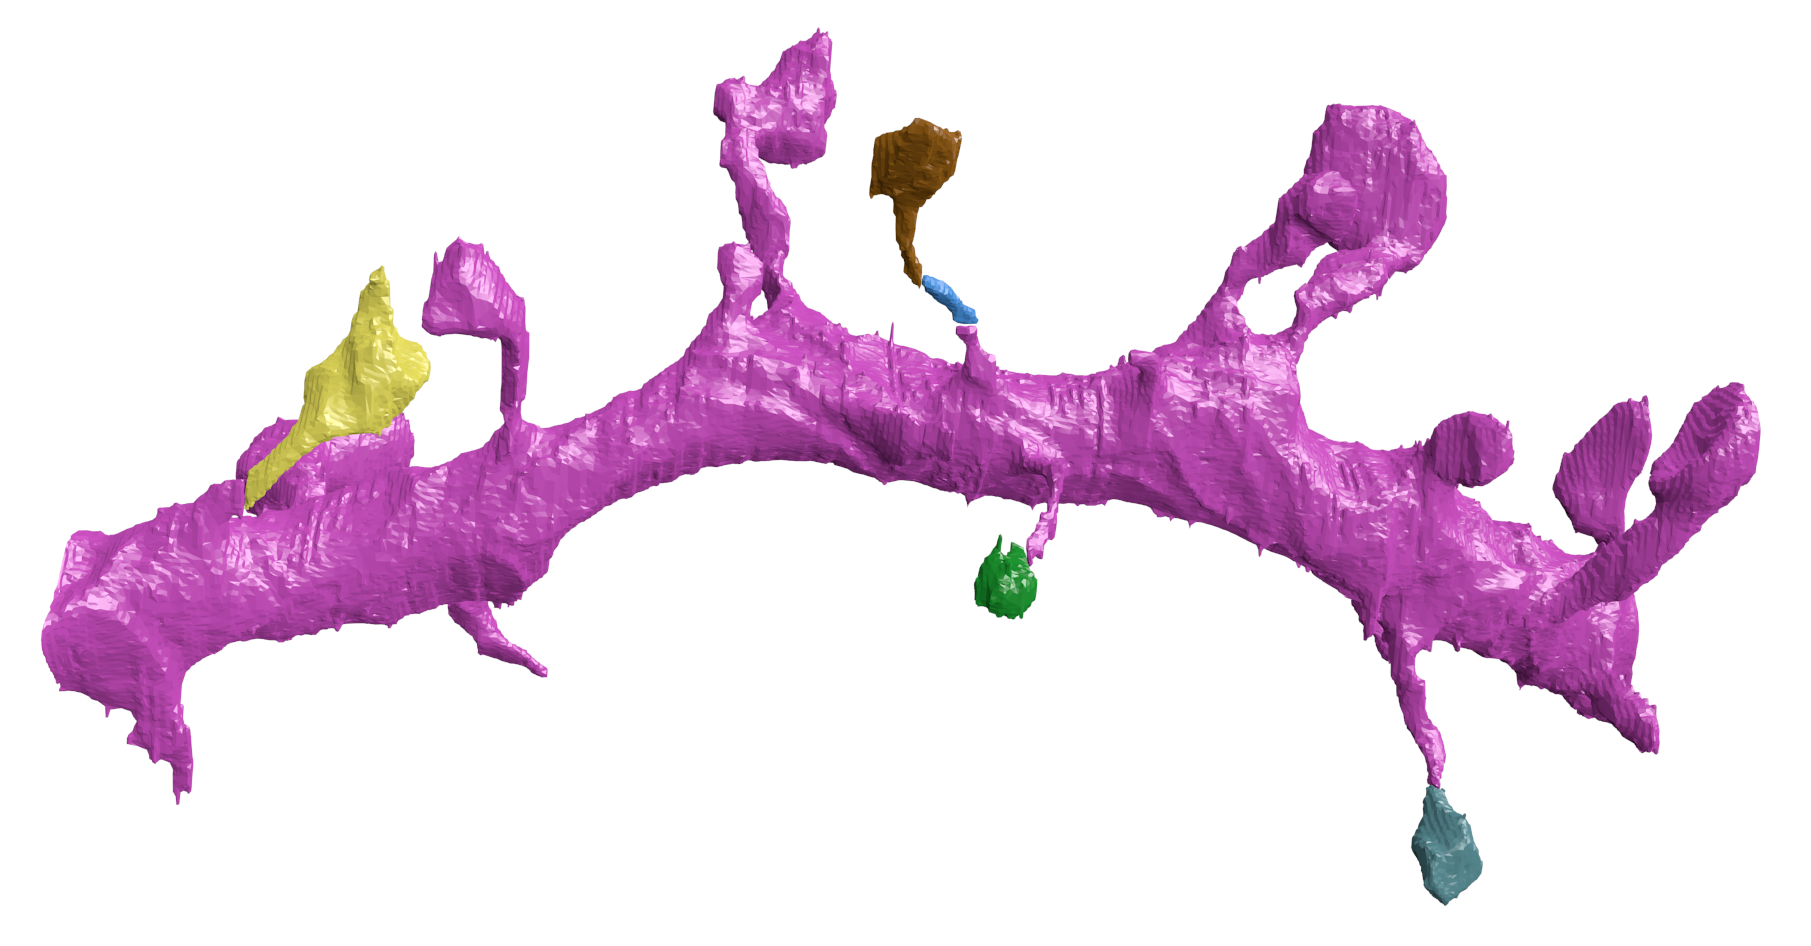
\includegraphics[width=0.85\linewidth]{./figures/VI-results/multicut-correct3.png}
		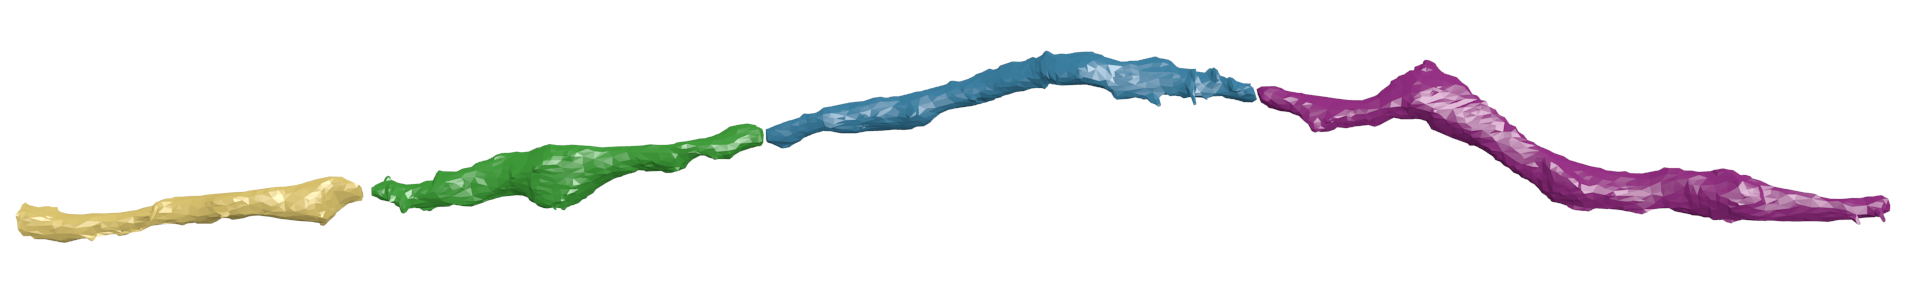
\includegraphics[width=0.85\linewidth]{./figures/VI-results/multicut-correct4.png}
		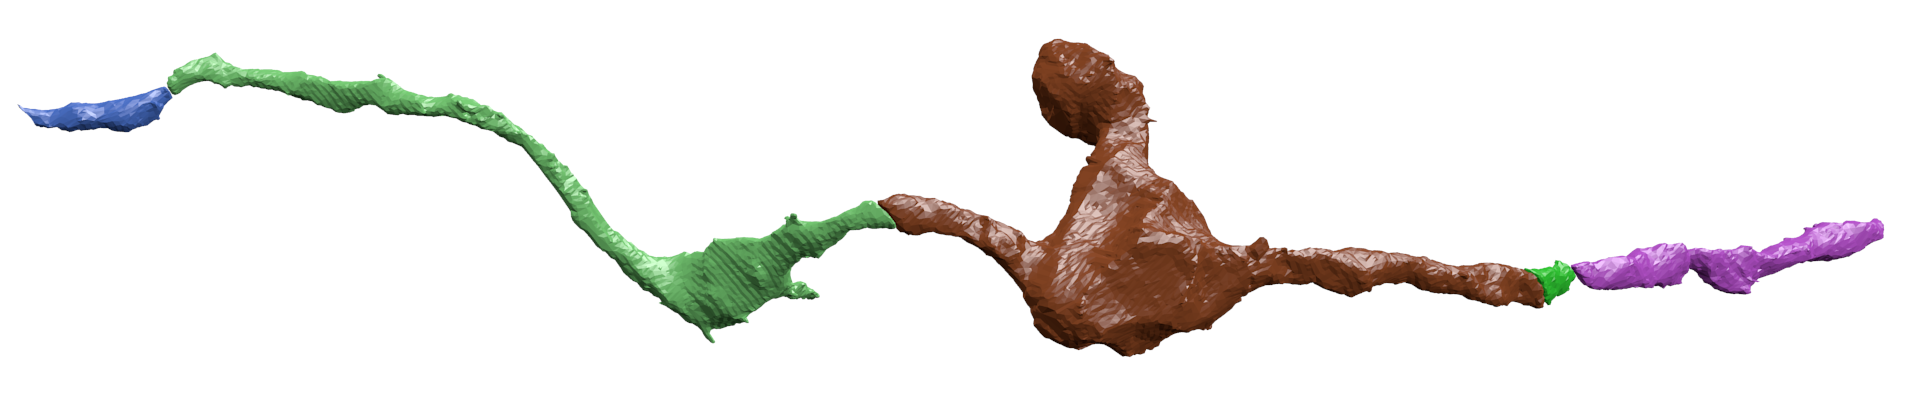
\includegraphics[width=0.85\linewidth]{./figures/VI-results/multicut-correct5.png}
	\end{minipage}
	\begin{minipage}{0.45\linewidth}
		\centering
		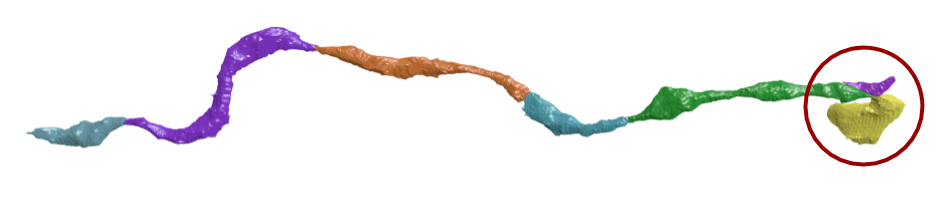
\includegraphics[width=0.85\linewidth]{./figures/VI-results/multicut-incorrect1.png}
		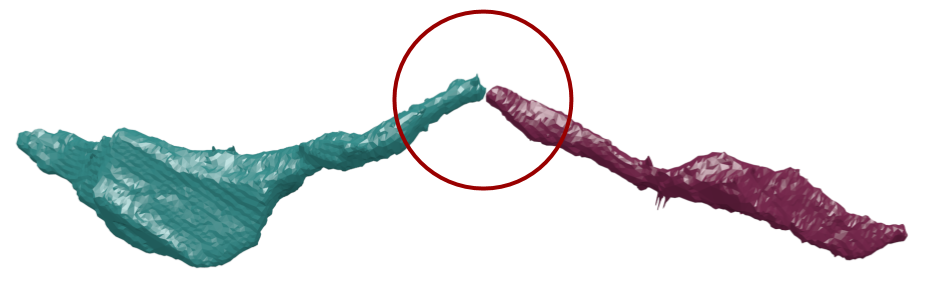
\includegraphics[width=0.85\linewidth]{./figures/VI-results/multicut-incorrect2.png}
		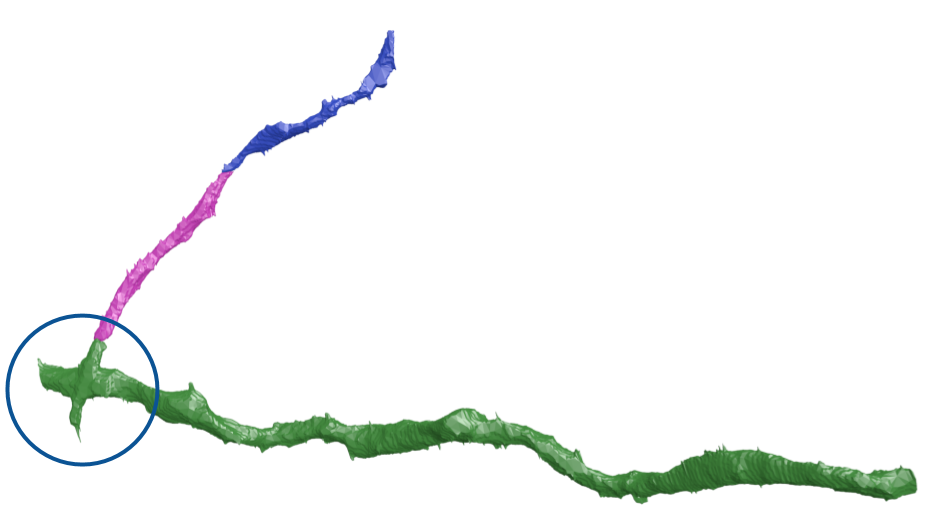
\includegraphics[width=0.85\linewidth]{./figures/VI-results/multicut-incorrect3.png}
		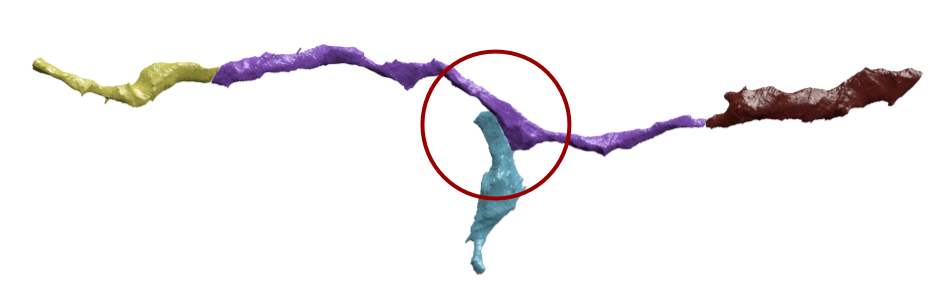
\includegraphics[width=0.85\linewidth]{./figures/VI-results/multicut-incorrect4.png}
	\end{minipage}
	\caption{(left) Segments of neurons before they were correctly merged by our method. (right) Circles indicate areas of wrong merges by our method (red) or by the initial pixel-based segmentation (blue).}
	\label{fig:qualitative-results}
\end{figure}

\subsection{Graph Pruning Results}

Table \ref{table:skeletonization} shows the results of pruning the skeleton graph using the algorithm discussed in Sec.~\ref{sec:skeletonization}. 
This edge pruning is essential for the graph partitioning algorithm, which has a computational complexity dependence on the number of edges. 
The baseline algorithm considers all adjacent regions for merging. 
Our method removes a significant portion of these candidates while maintaining a large number of the true merge locations (e.g., \TODO{XXX} compared to \TODO{XXX}). 
Our pruning heuristic removes at least $\TODO{X}\times$ the number of edges on all datasets, achieving a maximum removal rate of $\TODO{XX}\times$.
However, there are some adjacent over-segmented labels which are considered. 
Table~\ref{table:skeletonization} shows the results for our edge generation including the number of missed neighbors and potential penalty in VI score.
We present additional analysis of the skeletonization parameters in the supplemental material.

\begin{table}
	\centering
	\small
	\setlength{\tabcolsep}{0.75em}
	\begin{tabular}{c c c c} \hline
		\textbf{Dataset} & \textbf{Segment Adjacency} & \textbf{Skeleton Pruning} & \textbf{Missed Split Errors} \\ \hline
		Kasthuri &  & & \\
		FlyEM &  &  & \\
		FIB-25 &  & & \\ \hline
	\end{tabular}
	\caption{The results of our graph pruning approach compared to the baseline graph with all adjacent regions. We show the number of true merge locations (e.g., \TODO{XXX}) compared to total number of edges in the graph (e.g., \TODO{XXXXX}) for each case. The number of missed splits corresponds to the number of split errors that our method misses compared to an adjacency matrix.}
	\label{table:skeletonization}
\end{table}

We generate edges in our graph by using information from the skeletons. 
In particular, we do not enforce the constraint that edges in our graph correspond to adjacent segments.
Although neurons are continuous, the EM images often have noisy spots which cause an interruption in the input segmentation.
We still want to reconstruct these neurons despite the fact that the initial segmentation is non-continuous. 
The second and fourth examples in Fig.~\ref{fig:qualitative-results} show correctly reconstructed neurons where two of the segments are non-adjacent. 
On average in our datasets we correctly merge \TODO{XX} number of non-adjacent segments. 

There are some pairs of segments which we do not consider for merging because of our reliance on the skeletons.
Fig.~\ref{fig:skeleton-results} shows two such cases. 
The endpoints of both segments are circled.
In this example the small segment is carved from the larger segment in a location where there are no skeleton endpoints. 
There are on average $\TODO{XX}$ such examples in our datasets, corresponding to $\TODO{XX}$ in the variation of information split score. 

\begin{figure}[t!]
	\centering
	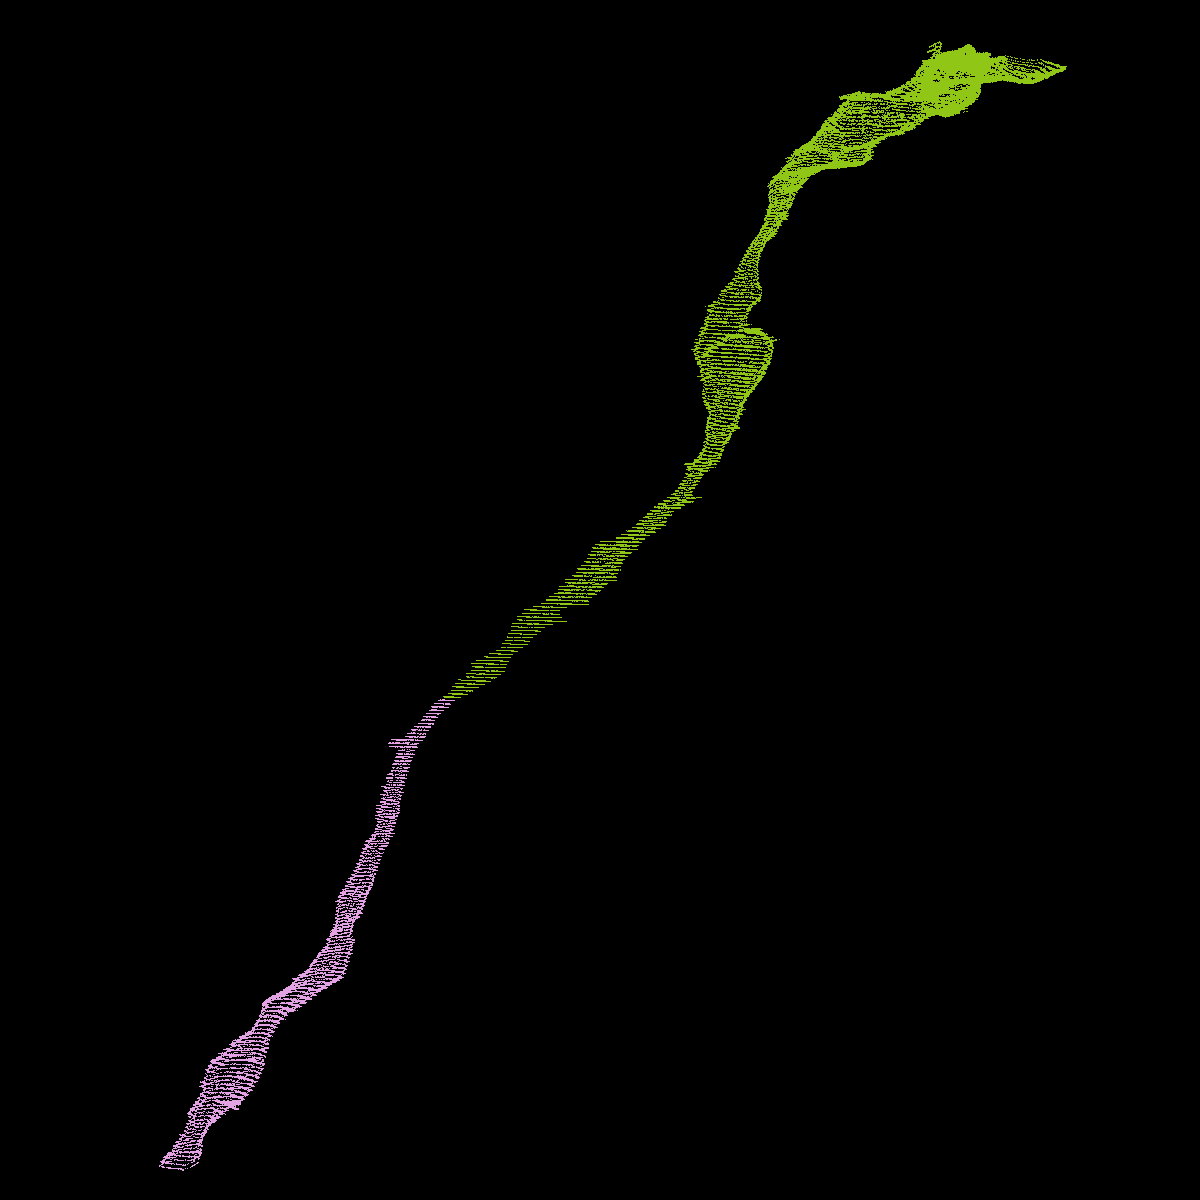
\includegraphics[width=0.45\linewidth]{./figures/merge_candidate1.png}		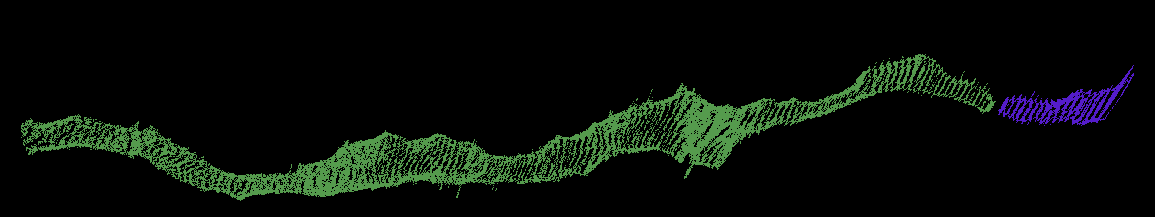
\includegraphics[width=0.45\linewidth]{./figures/merge_candidate2.png}
	\caption{Two example segment pairs that we incorrectly prune from our graph. The distances between the circled endpoints are greater than our thresholds.}
	\label{fig:skeleton-results}
\end{figure}

\subsection{CNN Classification Results}

\subsubsection{Inference Augmentation}

Data augmentation at test time can improve accuracy results~\cite{zeng2017deepem3d,lee2017superhuman}.
When computing the probability to merge two segments, we input the initial segment into our CNN as well as 3 randomly rotated and flipped examples (in the same manner as training augmentation).
This produces some additional increase in overall accuracy (Figure ~\ref{fig:receiver-operating-characteristic}).
The supplemental material contains experiments showing the trade-offs between increased accuracy and runtime when using these augmentation strategies.

Fig.~\ref{fig:receiver-operating-characteristic} shows the receiver operating characteristic (ROC) curve of our CNN classifier for all test datasets.
As shown by the ROC curve, the test results on the Kasthuri data are better than the results for FlyEM.
We believe this is in part because of the differences in the datasets (i.e., isotropy and $xy$ resolution).



\begin{figure}
	\centering
	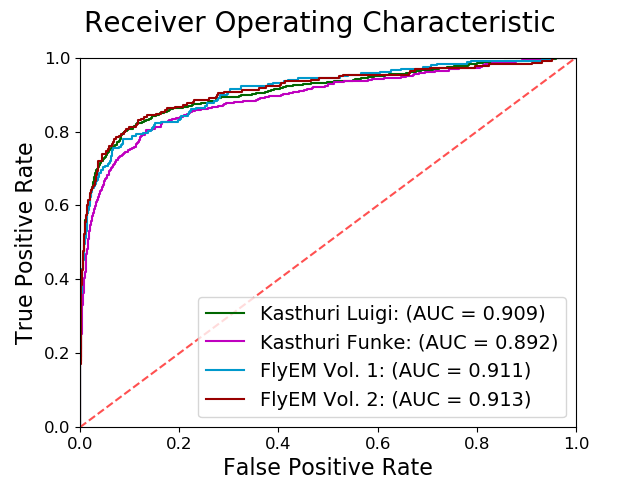
\includegraphics[width=0.45\linewidth]{./figures/receiver-operating-characteristic.png}		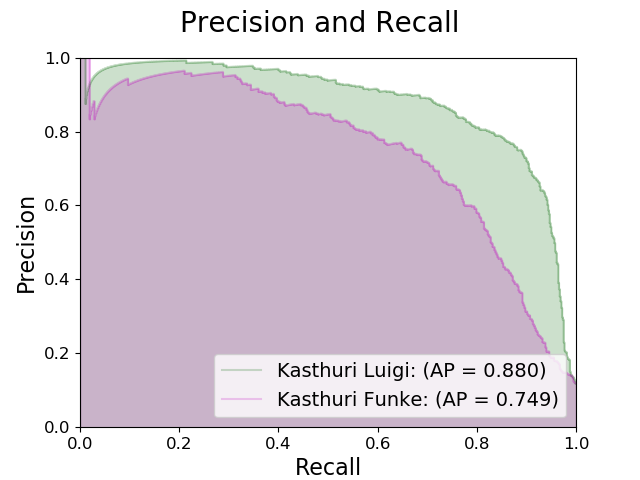
\includegraphics[width=0.45\linewidth]{./figures/precision-and-recall.png}
	\caption{The receiver operating characteristic (ROC) curves of our classifier on three connectomics datasets. The classifier works best on previously unseen data of the Kasthuri volume. The dashed blue line indicates better performance on the FlyEM datasets with retraining compared to without (solid blue).}
	\label{fig:receiver-operating-characteristic}
\end{figure}

\subsubsection{Generalization to Other Datasets}

Our neural network does not take as input the images or affinities to allow us to transfer network weights from one dataset to the next.
Table~\TODO{X} shows the result when training on the FlyEM data and inferring on the Kasthuri data and vice versa.
The classification results are reasonable despite the fact that the datasets vary in resolution and even animal type.


\subsection{Graph Optimization Results}

The graph optimization strategy using multicut increases our accuracy over using just the CNN.
Table \ref{table:multicut} shows the changes in precision, recall, and accuracy for all four datasets compared to the CNN with both the multicut and ``lifted'' multicut formulations.
These results correspond to $\beta = 0.5$ (Sec.~\ref{sec:edge-weights}). 
The precision increases on each dataset, although the recall decreases on all but one of the datasets.
The ``lifted'' variant further accentuates this trend of increasing precision and accuracy at the expense of recall. 
Since it is more difficult to correct merge errors than split errors, it is often desirable to sacrifice recall for precision.
Over the three testing datasets, applying a graph-based partitioning strategy reduced the number of merge errors by \TODO{XX}\%, \TODO{XX}\% and \TODO{XX}\%, respectively. 

\begin{table}[h]
	\centering
	\small
	\setlength{\tabcolsep}{0.3em}
	\begin{tabular}{c c c c | c c c} \hline
		& \multicolumn{3}{c}{\textbf{Multicut}} & \multicolumn{3}{c}{\textbf{Lifted Multicut}} \\ \hline
		\textbf{Dataset} & $\Delta$ \textbf{Precision} & $\Delta$ \textbf{Recall} & $\Delta$ \textbf{Accuracy} & $\Delta$ \textbf{Precision} & $\Delta$ \textbf{Recall} & $\Delta$ \textbf{Accuracy} \\ \hline
		Kasthuri Training & +3.61\% & -0.53\% & +0.60\% & +3.61\% & -0.53\% & +0.60\% \\
		Kasthuri Vol. 2 & +7.59\% & -1.77\% & +1.38\%  & +7.59\% & -1.77\% & +1.38\% \\
		FlyEM Vol. 1 & +2.68\% & +0.76\% & +0.66\% & +2.68\% & +0.76\% & +0.66\% \\
		FlyEM Vol. 2 & +2.22\% & -1.05\% & +0.29\% & +2.22\% & -1.05\% & +0.29\% \\ \hline
	\end{tabular}
	\caption{Precision, recall, and accuracy changes between CNN only and CNN paired with graph-optimized reconstructions for the training and three test datasets. The combined method results in better precision and accuracy.}
	\label{table:multicut}
\end{table}

Our post-processing method to agglomerate segments while enforcing the acyclic nature of our graph additionally improves precision by $\TODO{XX}\%$ on average while only costing $\TODO{XX}\%$ in recall. 
Note that our post-processing strategy by design cannot increase the recall. 

\subsection{Computational Performance}

\subsubsection{System} All performance experiments ran on an Intel Core i7-6800K CPU 3.40 GHz with a Titan X Pascal GPU. All code is written in Python and will be freely available upon paper decision. We use the Keras deep learning library for our neural networks with Theano backend and cuDNN 7 acceleration for CUDA 8.0.


\section{Conclusions}




{\small
\bibliographystyle{ieee}
\bibliography{paper}}

\end{document}
